\documentclass[letterpaper]{article}
\usepackage{geometry}
\usepackage{multicol}
\usepackage{minted}
\usepackage{amsmath, dsfont, mathtools, amssymb}
\usepackage{fontspec}
\usepackage{xcolor}
\usepackage{wrapfig}
\usepackage{graphicx}
\usepackage{soul}
\usepackage{enumitem}

\pagestyle{empty}
\geometry{top=0.5cm, bottom=0.5cm, left=0.5cm, right=0.5cm} 

\setlength{\columnsep}{1pt} % Remove space between columns
\setlength{\tabcolsep}{2pt} 


% Redefine section commands to use less space
\makeatletter
\renewcommand{\section}{\@startsection{section}{1}{0mm}%
                                {-1ex plus -.5ex minus -.2ex}%
                                {0.5ex plus .2ex}%
                                {\normalfont\tiny\bfseries
                                 \setlength{\fboxsep}{1pt}%
                                 \setlength{\fboxrule}{0.5pt}%
                                 \colorbox{pink}}}
% \renewcommand{\subsection}{\@startsection{subsection}{2}{0mm}%
%                                 {-1explus -.5ex minus -.2ex}%
%                                 {0.5ex plus .2ex}%
%                                 {\normalfont\normalsize\bfseries}}
% \renewcommand{\subsubsection}{\@startsection{subsubsection}{3}{0mm}%
%                                 {-1ex plus -.5ex minus -.2ex}%
%                                 {1ex plus .2ex}%
%                                 {\normalfont\small\bfseries}}
\makeatother

% Don't print section numbers
\setcounter{secnumdepth}{0}
\setlength{\parindent}{0em}
\setlength{\parskip}{0.2em}
\setlist[enumerate]{noitemsep, topsep=0pt, leftmargin=*}
\setlist[itemize]{noitemsep, topsep=0pt, leftmargin=*}
\newcommand{\mathcolorbox}[2]{\colorbox{#1}{$\displaystyle #2$}}


\begin{document}

\tiny

\begin{multicols*}{3}
    $P(n, r)=\frac{n !}{(n-r) !}\quad C(n, r)=\frac{n !}{r !(n-r) !}$

    $\log_a N = x, a^x = N, a^{\log_a N} = N$

    $g(n) \in O(f(n)) \text{if} \exists c > 0, n_0 > 0$ s.t. $\forall n \geq n_0, g(n) \leq c \cdot f(n)$

    $g(n) \in \Omega(f(n)) \text{if} \exists d > 0, n_0 > 0$ s.t. $\forall n \geq n_0, g(n) \geq d \cdot f(n)$

    $g(n) \in \Theta(f(n)) \text{if} \exists c, d > 0, n_0 > 0$ s.t. $\forall n \geq n_0, d \cdot f(n) \leq g(n) \leq c \cdot f(n)$

    $g(n) \in o(f(n)) \text{if} \forall c > 0, \exists n_0 > 0$ s.t. $\forall n \geq n_0, g(n) \leq c \cdot f(n)$

    $g(n) \in \omega(f(n)) \text{if} \forall d > 0, \exists n_0 > 0$ s.t. $\forall n \geq n_0, g(n) \geq d \cdot f(n)$

    \begin{itemize}
        \item $f(n)\in\Theta(g(n)) \to 2^{f(n)}\in\Theta(2^{g(n)})$ is false because $2^{n}\in\Theta(2^{n})$ but $2^{n}\notin\Theta(2^{n+1})$
    \end{itemize}

    \hl{Master theorem long}: Let $a\geq 1$ and $b>1$ be constants, let $f(n)$ be a function, and let
    \[T(n)=a T\left(\frac{n}{b}\right)+f(n)\]
    \begin{enumerate}
        \item If $f(n) \in O\left(n^{\log_b a-\epsilon}\right)$ for some $\epsilon>0$, then $T(n) \in \Theta\left(n^{\log_b a}\right)$.
        \item If $f(n) \in \Theta\left(n^{\log_b a}\right)$, then $T(n) \in \Theta\left(n^{\log_b a} \log n\right)$.
        \item If $f(n) \in \Omega\left(n^{\log_b a+\epsilon}\right)$ for some $\epsilon>0$, and if $a f\left(\frac{n}{b}\right) \leq c f(n)$ for some constant $c<1$ and all sufficiently large $n$, then $T(n) \in \Theta(f(n))$.
    \end{enumerate}

    \hl{Master theorem short}: For $T(n) = a\cdot T(\frac{n}{b}) + f(n),\quad T(1) = c,\quad a, c > 0,\ b > 1,\ f(n)\in \Theta(n^k),\ d\geq 0$, we have:
    \[T(n) = \begin{cases}
            \Theta(n^{\log_b a}) & \text{if } a > b^k \\
            \Theta(n^k \log n)   & \text{if } a = b^k \\
            \Theta(n^k)          & \text{if } a < b^k
        \end{cases}\]

    Doesn't apply to following cases:

    \begin{itemize}
        \item $T(n) = 2nT\left(\frac{n}{2}\right) + 1$ [$a = 2n$ is not a constant]
        \item $T(n) = \frac{1}{2}T\left(\frac{n}{2}\right) + 1$ [$a = \frac{1}{2}$ is not $\geq 1$]
        \item $T(n) = 2T(n) + 1$ [$b = 1$ is not $> 1$]
        \item $T(n) = T\left(\frac{n}{2}\right) - n\log n$ [$f(n) = -n\log n$ is not positive]
        \item $T(n) = T(n-1) + 1$ [recurrence is not in the right form]
        \item $T(n) = T\left(\frac{n}{2}\right) + T\left(\frac{n}{4}\right) + 1$ [recurrence is not in the right form]
    \end{itemize}

    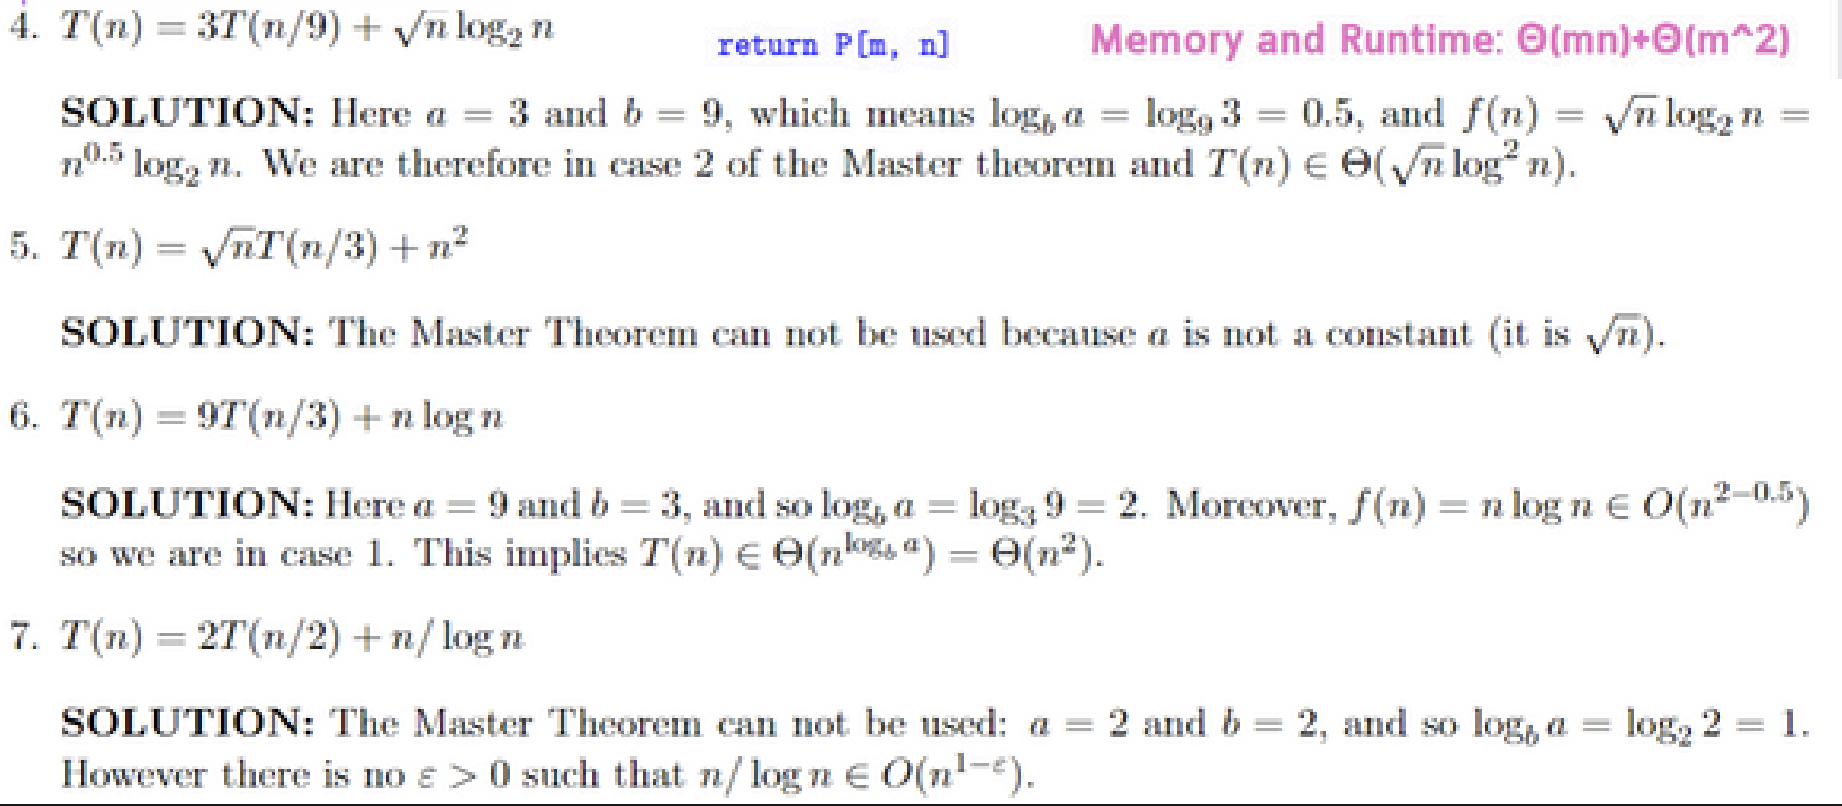
\includegraphics[width=\linewidth]{sheetimages/masterexample.png}

    $T(n)=2T(n/2)+n\cdot\log n$:

    \textbf{SOLUTION}: The Master Theorem cannot be used: $a=2, b=2, f(n)=n\log n$. Here, $n^{\log_b a} = n^{\log_2 2} = n^1 = n$. Using the long form the of Master Theorem, we have $f(n) = n log n \in \Omega(n^{1+\epsilon})$ for $\epsilon = 0.1$.

    Regularity LHS: $a f(n/b) = 2 \cdot (n/2) \log(n/2) = n \log(n/2) = n \log n - n$

    Regularity condition: $n \log n - n \leq c \cdot n \log n \to \log n\leq\frac1{1-c}$. As $n\to\infty$, $\log n \to \infty$, so the inequality cannot hold for any constant $c < 1$. Therefore, we cannot apply the Master Theorem to this recurrence.

    \hl{Series}:
    \[\begin{aligned}\sum_{i=0}^{n-1}ar^i&=a\left(\frac{1-r^n}{1-r}\right)&\sum_{i=0}^\infty ar^i&=\frac{a}{1-r}\text{ if }|r|<1\\\sum_{i=1}^ni&=\frac{n(n+1)}{2}&\sum_{i=1}^ni^2&=\frac{n(n+1)(n+2)}{6}\end{aligned}\]

    \section{P/NP/NPC/NPH}

    \begin{itemize}
        \item \textbf{Decision prob.}: A problem with a YES/NO answer, \textbf{Optimization prob.}: A problem that requires finding the best solution according to some criteria.
        \item P = \{problems solvable in polynomial time\}, NP = \{problems verifiable in polynomial time\},
        \item \textbf{Reduction}:
              \begin{itemize}
                  \item $X \leq_p Y$
                  \item $X \to Y$
                  \item Y at least as hard as X
                  \item $Y \in P/NP \to X \in P/NP$
                  \item $X \notin P/NP \to Y \notin P/NP$
              \end{itemize}
        \item NPC = \{$\forall X \in NP$: known NPC $\to X$ \}, NPH = \{ $\forall X: \forall Y \in NP : Y \to X \}$
        \item \textbf{Certificate}: A proposed solution to verify against to prove that a problem instance is a YES instance of the decision problem (in the context of NP).
              \\Examples:
              \begin{itemize}
                  \item For SAT: a truth assignment that satisfies the formula.
                  \item For Hamiltonian Cycle: a sequence of vertices representing the cycle.
                  \item For Subset Sum: a subset of numbers that sum to the target value.
                  \item For DS: A subset $D \subseteq V$ of size $k$ such that every vertex in $V$ is either in $D$ or adjacent to a vertex in $D$.
              \end{itemize}
        \item \textbf{Verifier}: An algorithm that verifies if a certificate is a correct solution to the problem instance.
    \end{itemize}
    \begin{itemize}
        \item If $P=NP$, then all NP problems (including SAT) are solvable in polynomial time
        \item If $P \ne NP$, then no NP-complete problem can be solved in polynomial time
        \item If problem A is NPC, B is special case of A: $B \to A \checkmark$: A least as hard as B
    \end{itemize}

    \begin{tabular}{|l|c|c|c|c|}
        \hline
                                                  & \textbf{P} & \textbf{NP} & \textbf{NPC} & \textbf{NPH} \\
        \hline
        \text{Solvable in $O(n^k)$}               & \checkmark &             &              &              \\
        \hline
        \text{Solution Verifiable in $O(n^k)$}    & \checkmark & \checkmark  & \checkmark   &              \\
        \hline
        \text{Reduces any NP Problem in $O(n^k)$} &            &             & \checkmark   & \checkmark   \\
        \hline
    \end{tabular}

    \hl{Proof NPC:} (1) Show $X \in NP$, (2) choose known NPC problem $Y$, (3) show $Y \to X$, (4) proof if I is a YES instance for X, then I' is YES for NPC and vice versa.

    \hl{Proof NP}: (1) Define certificate, (2) demonstrate how to verify certificate (3) show verifier runs in polytime.

    \hl{NP complete problems}:
    \begin{itemize}
        \item \textbf{Independent Set.} For a graph $G = (V,E)$, a subset of vertices $S \subseteq V$ is independent if no two vertices in $S$ are joined by an edge. Given a graph $G$ and $k \in \mathbb{N}$, does $G$ contain an independent set of size $k$ or larger?

        \item \textbf{Vertex Cover.} For a graph $G = (V,E)$, a subset of vertices $S \subseteq V$ is a vertex cover if every edge $e \in E$ has at least one of its endpoints in $S$. Given a graph $G$ and $k \in \mathbb{N}$, does $G$ contain a vertex cover of size $k$ or smaller?

        \item \textbf{Dominating Set.} For a graph $G = (V,E)$, a subset of vertices $S \subseteq V$ is a dominating set if every vertex $v \in V$ is either in $S$ or adjacent to at least one vertex in $S$. Given a graph $G$ and $k \in \mathbb{N}$, does $G$ contain a dominating set of size $k$ or smaller?

        \item \textbf{Set Packing.} Given an $n$-element set $U$, a collection of subsets $\{S_1, S_2, \ldots, S_m\} \subseteq U$ and a number $k \in \mathbb{N}$, does there exist a collection of at least $k$ of those sets with the property that no two of them intersect?

        \item \textbf{Set Cover.} Given an $n$-element set $U$, a collection of subsets $\{S_1, S_2, \ldots, S_m\} \subseteq U$ and a number $k \in \mathbb{N}$, does there exist a collection of at most $k$ of those sets whose union is equal to $U$?

        \item \textbf{Clique.} For a graph $G = (V,E)$, a subset of vertices $S \subseteq V$ is a clique if every pair of vertices in $S$ is joined by an edge. Given a graph $G$ and $k \in \mathbb{N}$, does $G$ contain a clique of size $k$ or larger?

        \item \textbf{Subset Sum.} Given a set of $n$ integers $V = \{v_1, v_2, \ldots, v_n\}$, is there a subset $U \subseteq V$ such that $\sum_{u_i \in U} u_i = k$?

        \item \textbf{Set Partition.} Given a set of $n$ integers $V = \{v_1, v_2, \ldots, v_n\}$, can the elements of $V$ be partitioned into two sets $U$ and $V \setminus U$ such that $\sum_{u_i \in U} u_i = \sum_{u_i \in V \setminus U} u_i$?

        \item \textbf{Graph Coloring.} A graph $G = (V,E)$ is said to be $k$-colorable if the endpoints of any edge $(u,v)$ can be colored using different colors when there is a total of $k$ available colors. Given a graph $G$ and $k \in \mathbb{N}$, does $G$ have a $k$-coloring?

        \item \textbf{3D Matching.} Given disjoint sets $X, Y, Z$ each of size $n$, and given a set $T \subseteq X \times Y \times Z$ of ordered triples, does there exist a subset of $n$ triples in $T$ such that each element of $X \cup Y \cup Z$ is contained in exactly one of those triples?

        \item \textbf{SAT (Satisfiability).}
              \begin{itemize}
                  \item Let $X = \{x_1, \ldots, x_n\}$ be a set of $n$ Boolean variables (i.e., each $x_i \in \{0,1\}$).
                  \item A term $t_i$ over $X$ is either one of the variables $x_i$ or its negation $\neg x_i$.
                  \item A clause $C_j$ of length $l$ is a disjunction of distinct terms: $C_j = t_1 \vee t_2 \vee \cdots \vee t_l$.
                  \item A collection of clauses is the conjunction $C_1 \wedge C_2 \wedge \cdots \wedge C_k$.
              \end{itemize}
              A truth assignment is an assignment of values of $0$ or $1$ to each $x_i \in X$ (i.e., a function $f : X \to \{0,1\}$). The collection of clauses $C_1 \wedge C_2 \wedge \cdots \wedge C_k$ is satisfiable if there exists a truth assignment that evaluates the collection to $1$. A problem is called $l$-SAT if the length of all clauses $C_j$ is exactly $l$.

        \item \textbf{3-SAT.} Given a collection of clauses over a set of Boolean variables $X$, where each clause has exactly three distinct terms, is the collection satisfiable?
        \item \textbf{Hamiltonian Cycle.} Given a graph $G = (V,E)$, does there exist a simple cycle that visits each vertex exactly once and returns to the starting vertex?
        \item \textbf{Traveling Salesman Problem (TSP).} Given a set of $n$ cities and a distance function $d(i,j)$ that gives the distance between each pair of cities $i$ and $j$, is there a tour that visits each city exactly once, returns to the starting city, and has total length at most $k$?
        \item \textbf{Steiner Tree.} Given a graph $G = (V,E)$ with edge weights and a subset of vertices $R \subseteq V$ called terminals, does there exist a subtree of $G$ that spans all terminals in $R$ and has total weight at most $k$?
        \item \textbf{Hitting Set.} Given a set $E^*$ with $n$ elements, and a collection $S = \{S_1, S_2, \ldots, S_m\}$ of subsets of $E^*$, a Hitting Set for $S$ is a subset $E' \subseteq E^*$ such that every $S_i$ contains at least one element of $E'$. For instance, if $E^* = \{a,b,c,d,e\}$ and the subsets of $E^*$ are $S_1 = \{a,b,d\}$, $S_2 = \{a,c\}$, $S_3 = \{a,d,e\}$, $S_4 = \{b,c,d\}$ and $S_5 = \{c,e\}$ then $\{b,c,e\}$ and $\{a,c\}$ are both hitting sets. The Minimum Hitting Set problem takes in the sets $E^*$ and $S$, and a positive integer $k$. The output should be \texttt{True} if $S$ admits a hitting set with at most $k$ elements, and \texttt{False} otherwise. In this question, you will design a polynomial-time reduction from Minimum Hitting Set to SAT.
    \end{itemize}

    \hl{Compare VS vs DS}:

    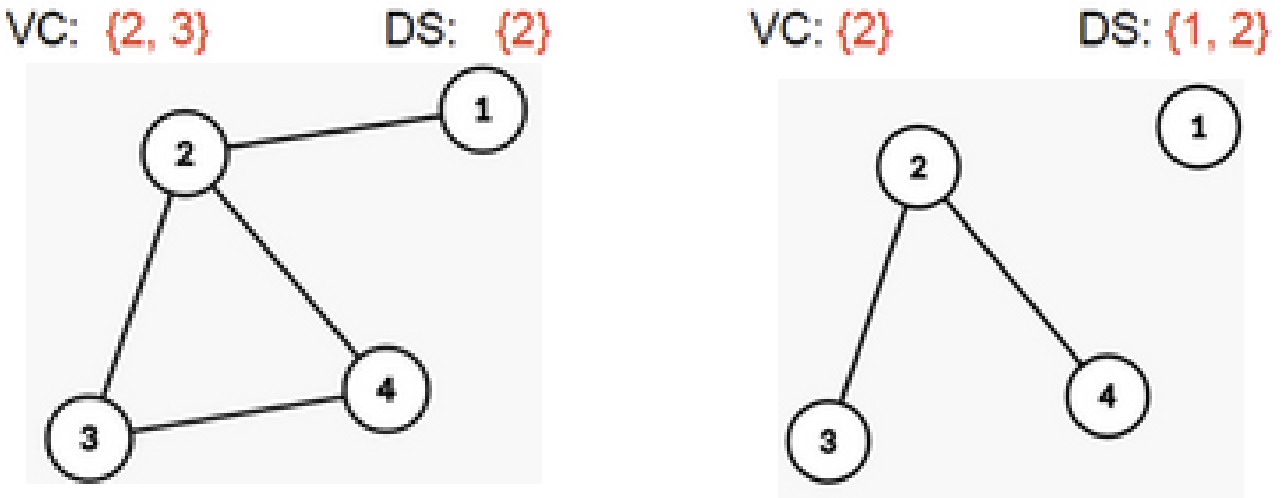
\includegraphics[width=.5\linewidth]{sheetimages/vsds.png}

    \hl{Some NP questions about reductions}


    \textbf{1. If $X \le_p X'$ and $X \in \mathbf{P}$, must $X' \in \mathbf{P}$?}
    \textbf{Status: Open Question.}

    \begin{itemize}
        \item It is easy to reduce an easy problem (e.g., interval scheduling, in $\mathbf{P}$) to a hard one (e.g., Maximum Independent Set, NP-complete).
        \item Such reductions can simply solve $X$ first, then output a trivial Yes/No instance of $X'$.
        \item Thus $X \in \mathbf{P}$ does \textit{not} imply $X'$ is easy.
        \item If we knew $\mathbf{P} \ne \mathbf{NP}$, the statement would be \textbf{false}, since $X'$ could be NP-complete.
        \item But since $\mathbf{P} = \mathbf{NP}$ is unresolved, this implication remains \textbf{open}.
    \end{itemize}

    \textbf{2. If $X \le_p X'$ and $X' \le_p X$, must both be NP-complete?}
    \textbf{Status: Open Question.}

    \begin{itemize}
        \item Two problems in $\mathbf{P}$ can reduce to each other trivially (solve one, output trivial instance of the other).
        \item If $\mathbf{P} \ne \mathbf{NP}$, neither is NP-complete.
        \item If $\mathbf{P} = \mathbf{NP}$, then every problem in $\mathbf{P}$ is NP-complete.
        \item Therefore, the statement depends on the unresolved $\mathbf{P}$ vs.\ $\mathbf{NP}$ question.
    \end{itemize}

    \textbf{3. If $X \le_p X'$ and $X \notin \mathbf{NP}$, must $X' \notin \mathbf{NP}$?}

    \begin{itemize}
        \item Suppose $X' \in \mathbf{NP}$.
        \item Let $f$ be the polynomial-time reduction from $X$ to $X'$.
        \item Because $X' \in \mathbf{NP}$, it has a polynomial-time verifier.
        \item Construct a verifier for $X$ by:
              \begin{enumerate}
                  \item Taking instance $I$ and certificate $C'$.
                  \item Computing $f(I)$.
                  \item Running the verifier for $X'$ on $(f(I), C')$.
              \end{enumerate}
        \item This proves $X \in \mathbf{NP}$, contradicting the assumption.
    \end{itemize}

    \textbf{Therefore, $X' \notin \mathbf{NP}$.}

    \textbf{4. Complement Problems: If $X \le_p X'$, must $\overline{X} \le_p \overline{X}'$?}
    \textbf{Answer: True.}

    \begin{itemize}
        \item A polytime reduction maps Yes-instances of $X$ to Yes-instances of $X'$ and
              No-instances to No-instances.
        \item The complement problem reverses Yes/No, but the same reduction still preserves correctness:
              $
                  I \in \overline{X} \iff I \notin X \iff f(I) \notin X' \iff f(I) \in \overline{X'}.
              $
        \item Thus the same reduction witnesses $\overline{X} \le_p \overline{X'}$.
    \end{itemize}

    \section{NPC reductions}

    \hl{3SAT to VC}:

    \textbf{Show that VC $\in$ NP.}

    Given a proposed set \(W\) of at most \(K\) vertices, we verify in polynomial time that every edge
    has at least one endpoint in \(W\).
    This is checked in \(O(mK)\) time. Thus VC is in NP.

    \textbf{Reduction}

    For the remainder of this tutorial, we will be reducing 3-SAT to vertex cover. Given an instance of 3-SAT with $n$ variables $X_1, \ldots, X_n$ and $m$ clauses $C_1, \ldots, C_m$, we construct a graph as follows:

    \begin{itemize}
        \item We generate $2n$ nodes called $X_1, \overline{X_1}, X_2, \overline{X_2}, \ldots, X_n, \overline{X_n}$ and $n$ edges $\{X_1, \overline{X_1}\}, \{X_2, \overline{X_2}\}, \ldots, \{X_n, \overline{X_n}\}$.

        \item We generate $3m$ nodes $Y_{1,1}, Y_{1,2}, Y_{1,3}, Y_{2,1}, Y_{2,2}, Y_{2,3},$ $\ldots, Y_{m,1}, Y_{m,2}, Y_{m,3}$ and 3m edges:
              $\{Y_{1,1}, Y_{1,2}\}, \{Y_{1,1}, Y_{1,3}\}, \{Y_{1,2}, Y_{1,3}\}$ $\ldots, \{Y_{m,1}, Y_{m,2}\}, \{Y_{m,1}, Y_{m,3}\}, \{Y_{m,2}, Y_{m,3}\}$.

        \item For each literal $\ell \in \{X_i, \overline{X_i}\}$ appearing at position $j$ in clause $C_k$, we add the edge $\{Y_{k,j}, \ell\}$.
    \end{itemize}

    \textbf{Choose \(K\) for the reduction.}

    We select
    $
        K = n + 2m,
    $
    where \(n\) is the number of variables and \(m\) the number of clauses.

    \textbf{If the 3-SAT instance is satisfiable, then the constructed graph has a VC of size at most \(K\).}

    Assume a satisfying assignment exists.

    \begin{itemize}
        \item For each variable \(X_i\), include exactly one of the pair \(\{X_i,\overline{X_i}\}\):
              include \(X_i\) if \(X_i\) is true, otherwise include \(\overline{X_i}\).
              This covers all variable-pair edges.

        \item For each clause \(C_j\), let the literal in position \(t\) be true.
              Include the two clause vertices \(Y_{j,k}\) with \(k\neq t\).
              These two vertices cover all three edges of the clause triangle.
    \end{itemize}

    This uses \(n\) variable vertices and \(2m\) clause vertices, totalling \(K=n+2m\).
    All edges are covered.

    \textbf{If the constructed graph has a VC of size at most \(K\), then the 3-SAT instance is satisfiable.}

    Suppose a VC \(W\) has size at most \(n+2m\).

    \begin{itemize}
        \item Each variable-pair edge \(\{X_i,\overline{X_i}\}\) must have at least one endpoint in \(W\),
              so for each \(i\), at least one of \(X_i,\overline{X_i}\) is chosen.

        \item Each clause triangle needs at least two of its vertices in the cover.
              Thus exactly \(2m\) of the chosen vertices must come from clause gadgets, leaving exactly \(n\) chosen variable-vertices.
              Hence for each variable, \emph{exactly one} of \(\{X_i,\overline{X_i}\}\) is in the cover.
    \end{itemize}

    Define the assignment:
    \[
        X_i = \text{True} \text{ if } X_i \in W,\qquad X_i = \text{False} \text{ if } \overline{X_i} \in W.
    \]

    In each clause, exactly one triangle node is \emph{not} selected in \(W\).
    Its incident literal-edge \(\{Y_{j,t},\ell\}\) must therefore be covered by the literal vertex \(\ell\),
    implying that literal is true.
    Thus every clause has a true literal, so the formula is satisfiable.


    \textbf{Conclusion.}
    The reduction is correct: the 3-SAT instance is satisfiable iff the constructed graph has a vertex cover of size at most \(K = n + 2m\).

    \hl{3SAT to ST}:

    \begin{minipage}{0.45\linewidth}
        Given the graph below, how do we connect the shaded parts (S) with least amount of edges? \underline{Optimization problem}, minimizing edges connecting.
    \end{minipage}
    \begin{minipage}{0.5\linewidth}
        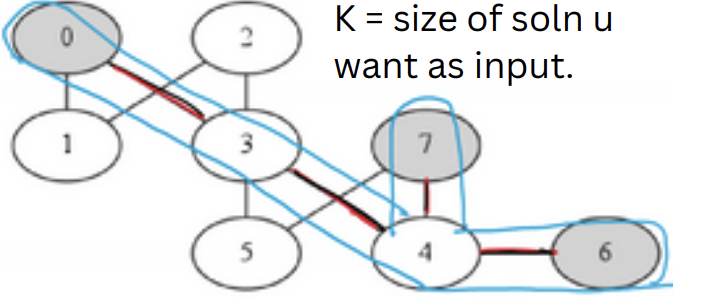
\includegraphics[width=\linewidth]{sheetimages/st.png}
    \end{minipage}

    \underline{Decision Problem}: Output can be either a yes or no. For Steiner, Yes is when it connects all shaded nodes, with edge amount < k. If u specify edge amount < any other solution, is bNOT a decision problem.

    Certifying the algorithm
    (1) Check that edges in E’ have size at most k, (2) the edges connect all shaded
    vertices with a DFS on the subgraph of G formed by deleting all edges but the ones
    in E’, starting from any shaded nodes. During DFS, we “check off” all shaded nodes.
    If |E’| <= K and all shaded notes are checked off, E’ is a good solution (Yes). is in
    class NP. If all nodes shaded the problem is MST algo.

    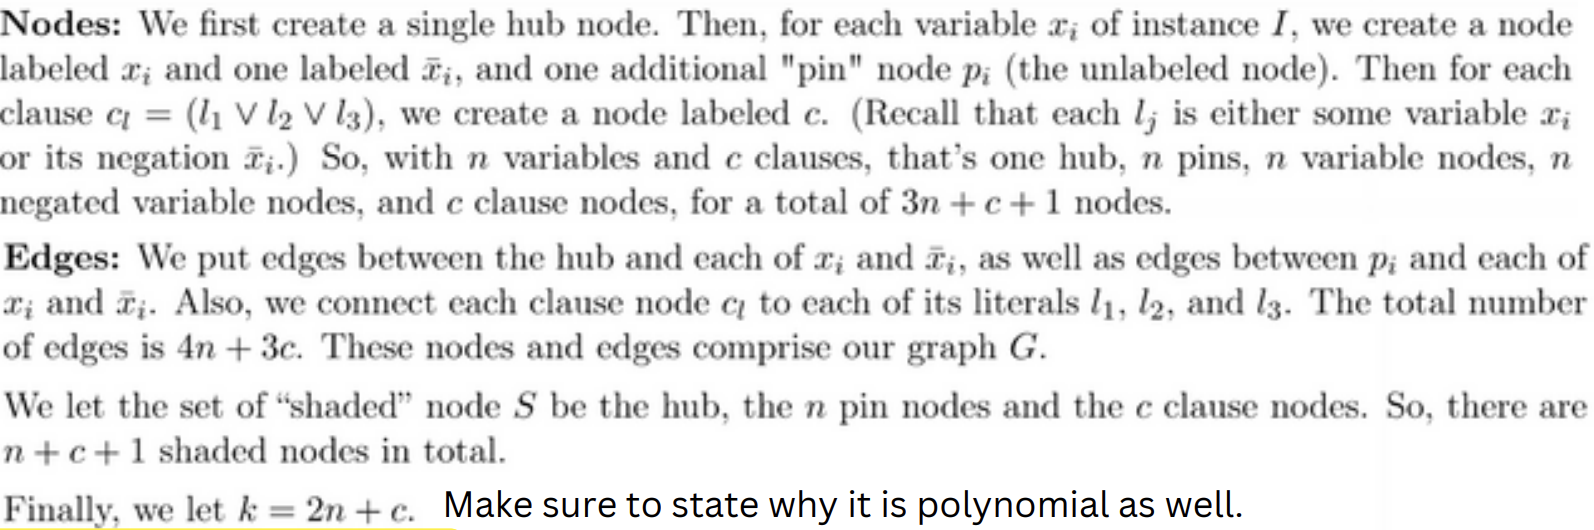
\includegraphics[width=\linewidth]{sheetimages/stconvert.png}

    \hl{SAT to 3SAT}:

    Consider a single original clause \(C\) containing \(k\) literals:

    Number of 3-clauses \(c(k)\), Number of fresh (new) variables \(v(k)\), Total number of literal occurrences \(L(k)\):

    $
        c(k)=
        \begin{cases}
            1,   & k=1 \lor k = 3, \\
            2,   & k=2,            \\
            k-2, & k\ge 4.
        \end{cases}$
    $v(k)=
        \begin{cases}
            1,   & k=1,    \\
            1,   & k=2,    \\
            0,   & k=3,    \\
            k-3, & k\ge 4.
        \end{cases}$
    $L(k)=3c(k)=
        \begin{cases}
            3,      & k=1 \lor k=3, \\
            6,      & k=2,          \\
            3(k-2), & k\ge 4.
        \end{cases}
    $

    \textbf{\underline{Reduction Construction}}

    Let a CNF formula $F$ be a conjunction of clauses. For each clause
    $C = (\ell_1 \vee \ell_2 \vee \cdots \vee \ell_k)$,
    construct an equivalent set of 3-literal clauses as follows.

    \textbf{Case 1: $k=3$.}
    Keep $C$ unchanged.

    \textbf{Case 2: $k=1$.}
    Introduce a fresh variable $z$ and replace $C=(\ell_1)$ with:
    $
        (\ell_1 \vee z \vee \neg z).
    $

    \textbf{Case 3: $k=2$.}
    Introduce a fresh variable $z$ and replace $C=(\ell_1 \vee \ell_2)$ with:
    $
        (\ell_1 \vee \ell_2 \vee z) \ \wedge\  (\ell_1 \vee \ell_2 \vee \neg z).
    $

    \textbf{Case 4: $k \ge 4$.}
    Introduce fresh variables $y_1,\dots,y_{k-3}$ and replace $C$ with the chain:
    $
        (\ell_1 \vee \ell_2 \vee y_1),
        (\neg y_1 \vee \ell_3 \vee y_2),
        \dots,
        (\neg y_{k-4} \vee \ell_{k-2} \vee y_{k-3}),
        (\neg y_{k-3} \vee \ell_{k-1} \vee \ell_k).
    $

    Let $F'$ be the conjunction of all replaced clauses.

    \textbf{\underline{Correctness Proof}}

    We show that $F$ is satisfiable iff $F'$ is satisfiable.

    \textbf{($\Rightarrow$) If $F$ is satisfiable, then $F'$ is satisfiable.}

    Let $\alpha$ satisfy $F$. Extend $\alpha$ to the fresh variables:

    \begin{itemize}
        \item For $k=1$: $(\ell_1 \vee z \vee \neg z)$ is satisfied regardless of $z$.
        \item For $k=2$: Since $(\ell_1 \vee \ell_2)$ is true, at least one of the two clauses is true for any $z$.
        \item For $k\ge 4$: If some $\ell_j$ is the first true literal, assign $y_1,\dots,y_{j-3}$ to be false and $y_{j-2}$ to be true, making the clause containing $\ell_j$ true and satisfying the chain.
    \end{itemize}

    Thus all clauses in $F'$ are satisfied.

    \textbf{($\Leftarrow$) If $F'$ is satisfiable, then $F$ is satisfiable.}

    Let $\beta$ satisfy $F'$. Consider any original clause $C=(\ell_1,\dots,\ell_k)$.

    \begin{itemize}
        \item $k=1$: $(\ell_1 \vee z \vee \neg z)$ can only be true if $\ell_1$ is true.
        \item $k=2$: If both $\ell_1$ and $\ell_2$ were false, the two clauses $(\ell_1 \vee \ell_2 \vee z)$ and $(\ell_1 \vee \ell_2 \vee \neg z)$ reduce to $z$ and $\neg z$, impossible. Hence $C$ is true.
        \item $k\ge 4$: Assume all $\ell_i$ are false. Then $C_1=(\ell_1 \vee \ell_2 \vee y_1)$ forces $y_1$ true.
              $C_2$ then forces $y_2$ true, and so on, implying $y_{k-3}$ true.
              The last clause $(\neg y_{k-3} \vee \ell_{k-1} \vee \ell_k)$ becomes false, contradiction.
              Thus some $\ell_i$ must be true.
    \end{itemize}

    Therefore every original clause of $F$ is true under $\beta$ restricted to the original variables.

    \hl{3-SAT $\le_p$ Independent Set}
    \begin{itemize}
        \item IS: A collection of vertices where no two vertices are directly connected by an edge.
        \item Given a 3-SAT instance with $k$ clauses, construct a graph $G$ with a triangle of 3 nodes for each clause (one node per literal).
        \item Add edges between any conflicting literals (e.g., $x$ and $\neg x$) across different triangles.
        \item $G$ has an Independent Set of size $k$ if and only if the 3-SAT formula is satisfiable. (Exactly one true literal per clause/triangle, no conflicting literals.)
    \end{itemize}

    \hl{3-SAT $\le_p$ Hamiltonian Cycle}
    \begin{itemize}
        \item Hamiltonian Cycle: visiting every node exactly once.
        \item Construct a graph with $2^n$ possible paths representing the $2^n$ truth assignments (using "ladder" structures for each variable).
        \item Insert "clause nodes" that can only be visited if the path traverses a specific variable ladder in the direction corresponding to the truth value that satisfies the clause.
        \item A Hamiltonian Cycle exists iff there is a truth assignment that allows visiting all clause nodes.
    \end{itemize}

    \hl{3-SAT $\le_p$ 3-Coloring}
    \begin{itemize}
        \item Create a "palette" triangle with nodes True, False, Base.
        \item For every variable, create a pair of connected nodes $(x_i, \neg x_i)$ connected to Base (forcing one to be True, one False).
        \item For each clause, attach a "gadget" subgraph that can only be 3-colored if at least one of its input literals is colored True.
    \end{itemize}

    \hl{3-SAT $\le_p$ Subset Sum}
    \begin{itemize}
        \item Generate numbers with many digits (essentially bitmasks).
        \item Each digit position corresponds to a variable or a clause.
        \item Selecting a number corresponds to setting a variable to True or False.
        \item The sum "target" $W$ forces exactly one assignment per variable and checks that each "clause digit" sums to a value indicating satisfaction.
    \end{itemize}

    % \hl{SAT $\le_p$ 3-SAT}
    % \begin{itemize}
    %     \item SAT asks if there is an assignment of truth values (True/False) to variables $X_1,\dots,X_n$ such that a collection of clauses (disjunctions of literals) are all True. It is NP-complete.
    %     \item Reduction (SAT to 3-SAT): General SAT can be reduced to 3-SAT to prove 3-SAT is hard.
    %     \item Length 1 (e.g., $X_5$): Replaced by 4 clauses using two new variables to force $X_5$ to be True.
    %     \item Length 2 ($X_2 \vee X_3$): Replaced by 2 clauses introducing one new variable.
    %     \item Length $>3$: A clause with $k$ literals is broken into $k-2$ clauses using $k-3$ new variables to link them.
    % \end{itemize}

    % \hl{3-SAT $\le_p$ Steiner Tree}
    % \begin{itemize}
    %     \item Given a graph $G = (V,E)$, a subset of vertices $S \subseteq V$ (terminals), and an integer $k$, determine if there is a subset of edges $E' \subseteq E$ with $|E'| \le k$ that connects all vertices in $S$.
    %     \item Gadgets: Uses a "hub" node and "variable gadgets" where picking a path corresponds to assigning True/False.
    %     \item Structure: Clause nodes are connected to their corresponding literal nodes.
    %     \item Constraints: Edge limit $k = 2n + c$ (where $n$ = variables, $c$ = clauses) to force selection of exactly one truth value per variable and at least one true literal per clause.
    % \end{itemize}

    \hl{Bipartite Matching $\le_p$ SAT}
    \begin{itemize}
        \item Determine if a graph $G = (V,E)$ is bipartite (can be split into two disjoint sets $U$ and $W$ with no internal edges).
        \item Variables: $X_i$ for each vertex. True = Set $U$, False = Set $W$.
        \item Clauses: For every edge $(u,v)$, add $(X_u \vee X_v) \wedge (\neg X_u \vee \neg X_v)$ to force $X_u \ne X_v$.
    \end{itemize}

    \hl{Very Visible Vertex Cover (V2VC)}
    \begin{itemize}
        \item Vertex cover where nodes cover edges up to distance 2.
        \item Proof (in NP): Certificate is subset $S$. Verifier checks if every edge is incident to a neighbor of $S$.
        \item Reduction (VC $\le_p$ V2VC): Subdivide every edge $(u,v)$ in VC instance by adding node $w$. New edges are $(u,w), (w,v)$. A V2VC on this new graph is equivalent to VC on original.
        \item Counter-Example: V2VC $\le_p$ VC is false. Complete graph $K_4$ needs 3 nodes for VC but only 2 for V2VC.
    \end{itemize}

    \hl{Independent Set to Clustering}
    \begin{itemize}
        \item Maximize the minimum similarity of an intra-category edge (partition into $k$ sets).
        \item Reduction: From Independent Set (partition into $k$ independent sets). Map graph $G$ to photos. If $(u,v) \in E$, similarity $S(u,v) = 0$. Else $S(u,v) = 1$. If MICS $\ge 1$, then all intra-category edges are non-edges in $G$, implying independent sets.
    \end{itemize}


    \section{Amortized analysis}

    $D_i = $ state of algo after $i$th operation. Potential: define s.t. $\Phi(D_0)=0, \Phi(D_i)\geq 0$

    $i$th op am cost: $\text{cost}_{am}(op_i) = \text{cost}_{real}(op_i) + \Phi(D_i) - \Phi(D_{i-1})$

    Cost of $n$ ops: $\sum_{i=1}^n \text{cost}_{am}(op_i) \geq \sum_{i=1}^n \text{cost}_{real}(op_i)$

    \hl{Array size change cost}

    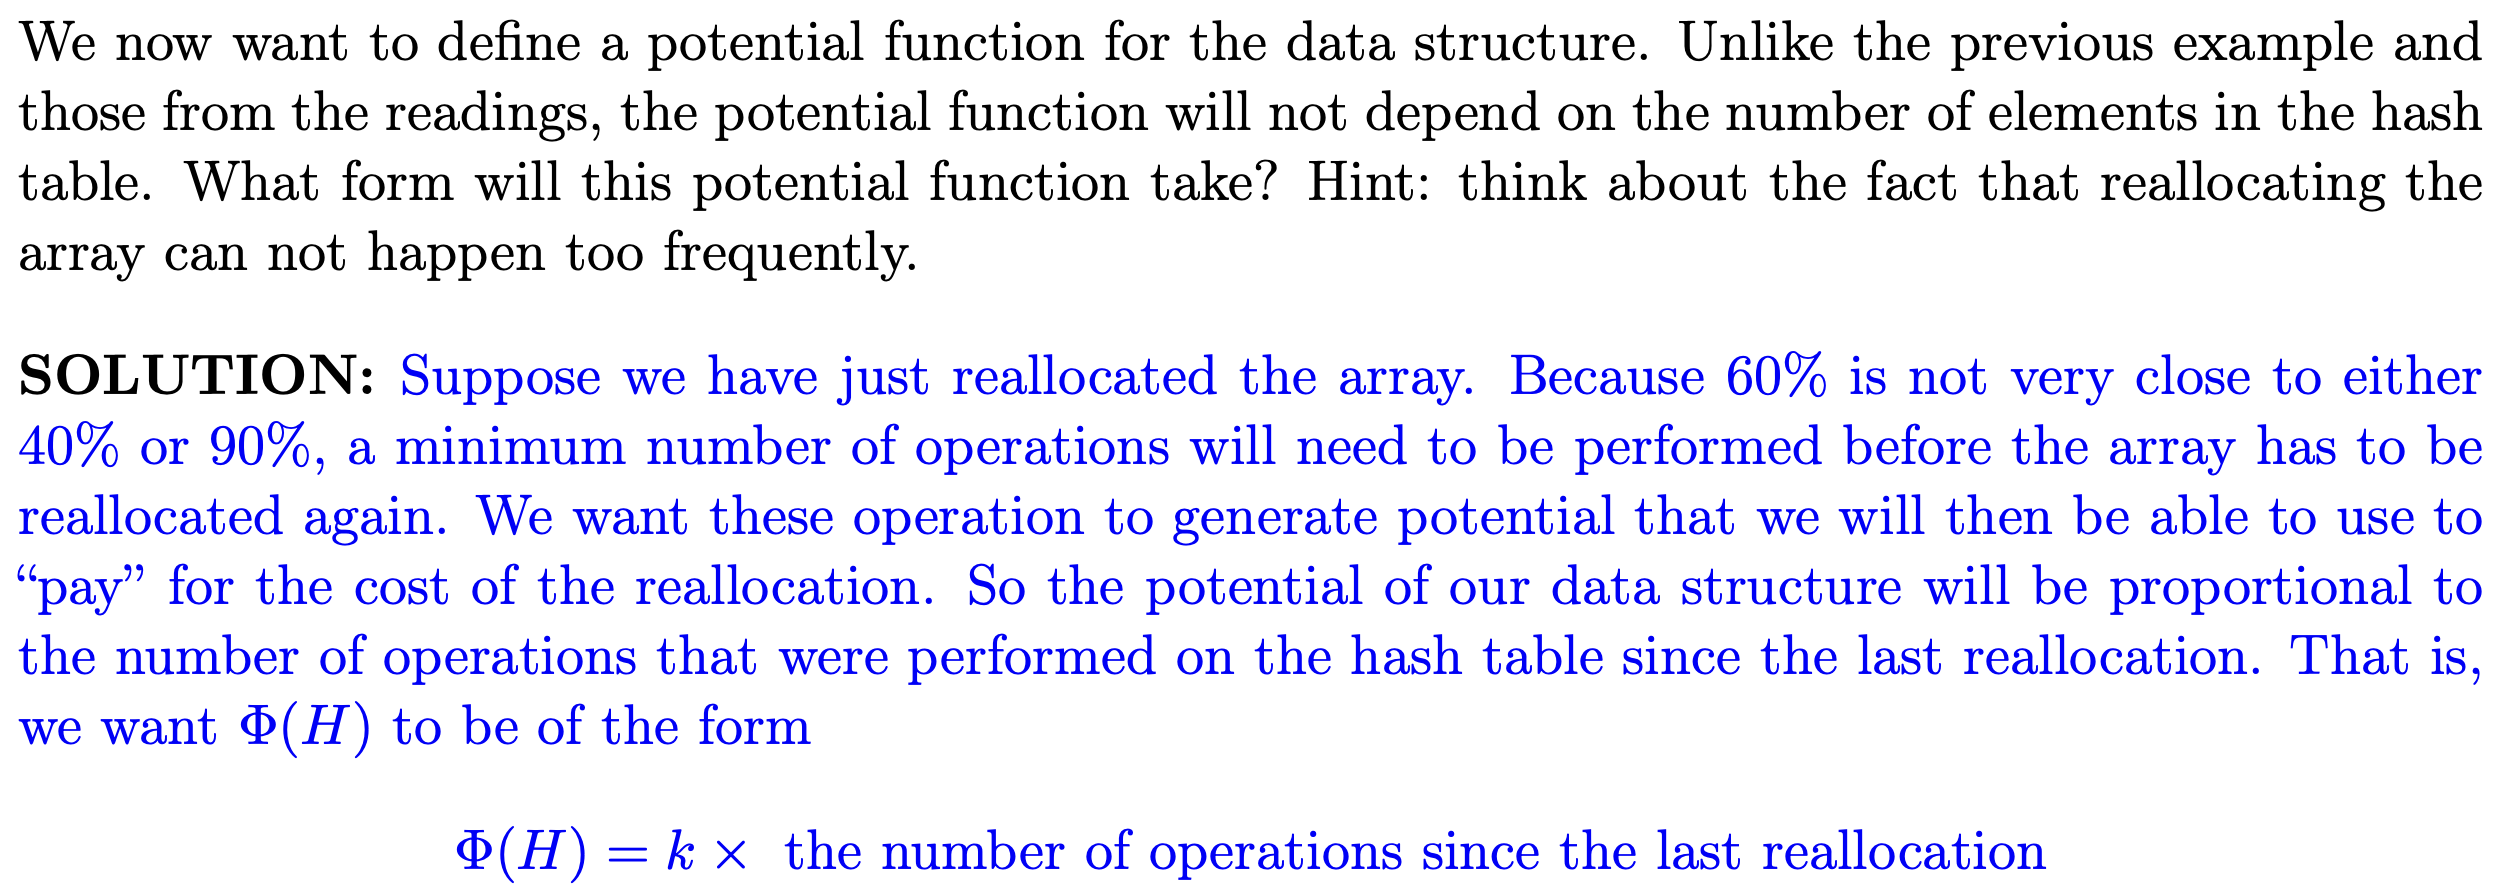
\includegraphics[width=\linewidth]{sheetimages/amor1.png}
    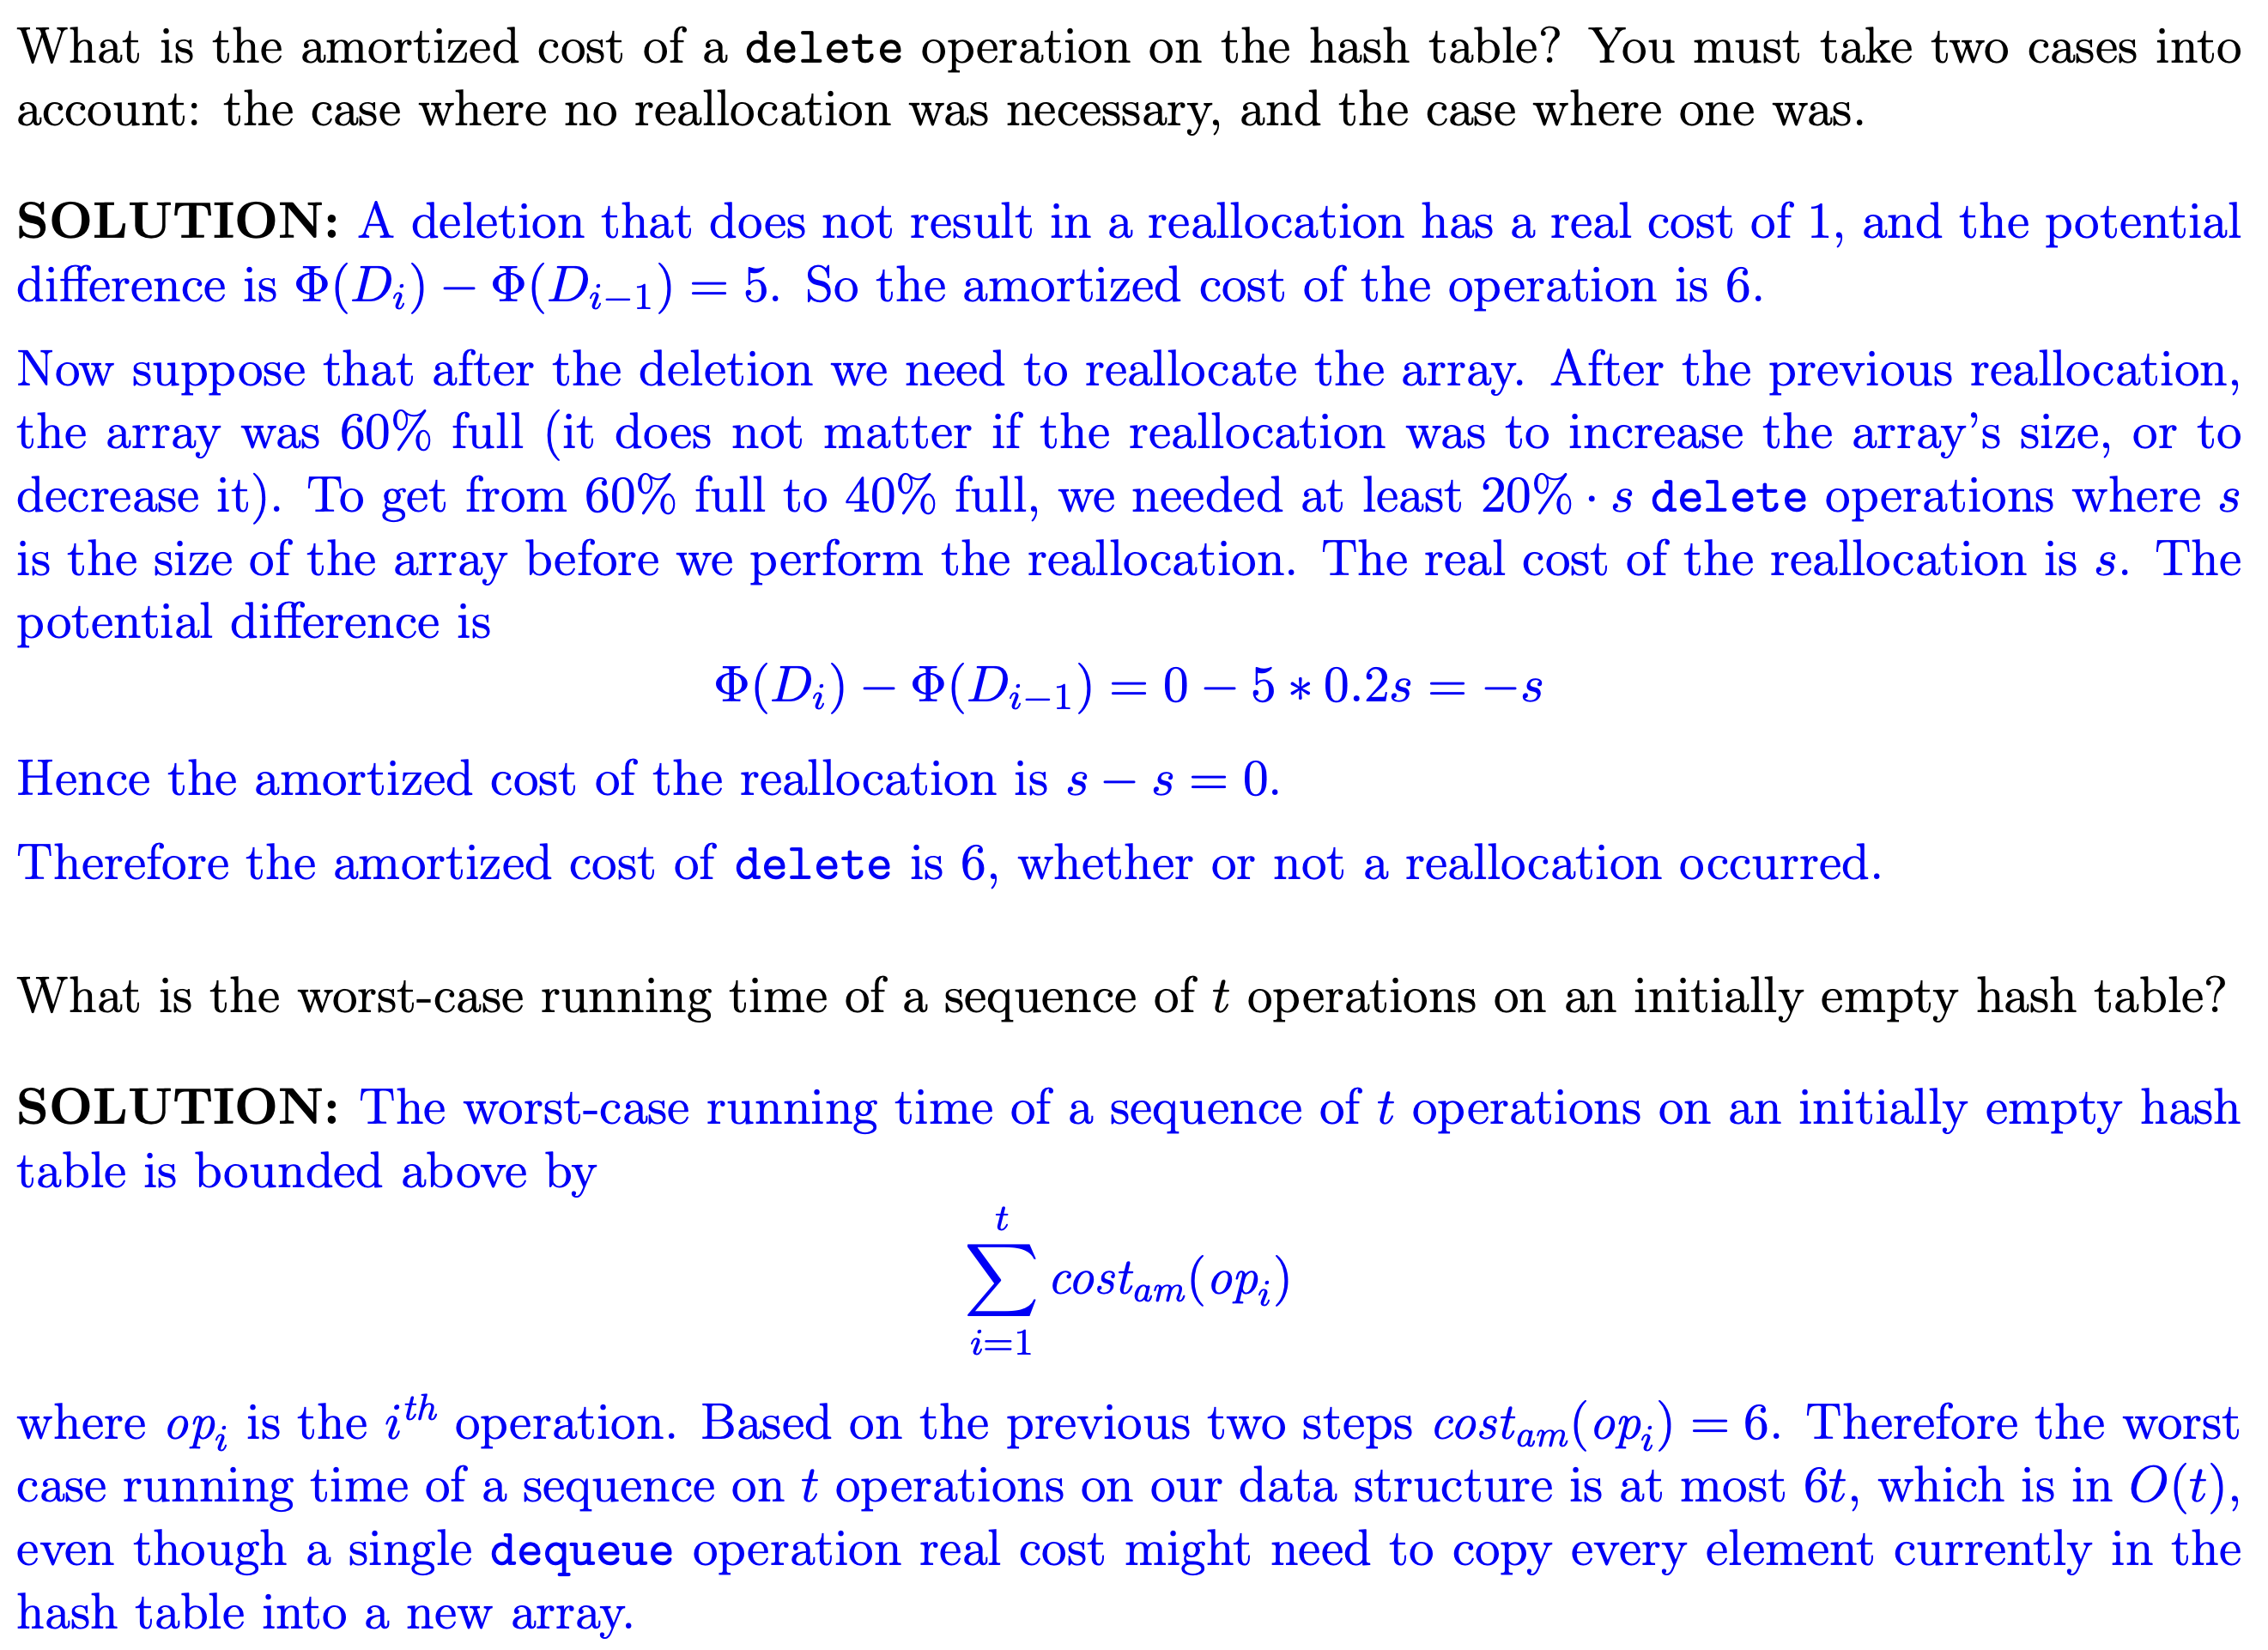
\includegraphics[width=\linewidth]{sheetimages/amor2.png}

    \hl{Counter}

    \textbf{Setup:} Binary counters as singly linked lists (LSB at head). Operations: Increment(C), Double(C), Add(C, C′). Potential: $\Phi(C) = \text{bits}(C) + \text{ones}(C)$.

    \textbf{1. Amortized cost of Double(C):}
    Real cost: 1 (prepend 0). Potential increase: 1. \textbf{Amortized cost: 2}

    \textbf{2. Amortized cost of Add(C, C′):} (C has $n$ bits, C′ has $n' \geq n$ bits)
    \begin{itemize}[noitemsep]
        \item Real cost: $O(n)$ for addition + carry propagation
        \item bits(C) decreases by $n-1$; bits(C′) increases by $\leq 1$
        \item ones bits: $\leq k$ ones change to zeros (except last), then $+1$
        \item Net: $\Delta\Phi = 1 - (n-1) + (k-1) - k + 1 = 2 - n$
    \end{itemize}
    \textbf{Amortized cost: } $n + (2-n) = 2$ (or at most 4 with loose bounds)

    \textbf{3. Tight bound for $n$ mixed operations:}
    Each operation has $O(1)$ amortized cost. Total amortized cost: $O(n)$. Since total real cost $\leq$ total amortized cost, worst-case running time is $\boxed{\Theta(n)}$.

    \section{Greedy}


    \hl{Greedy stays ahead proof}: \underline{Each step} \underline{\textbf{better}} than or equal to any other solution's step \underline{by induction}

    \hl{Exchange argument proof}: (1) Start from any sol (2) Series of exchanges that \textbf{doesn't undermine the quality of solution} (3) Arrive at greedy sol (4) Conclude sol greedy at least as good as any other

    \hl{Interval scheduling}: Given $n$ intervals with start times $s_i$ and finish times $f_i$, find a set of non-overlapping intervals with maximum cardinality.

    \begin{verbatim}
Sort intervals by increasing finish time
A = empty set
lastFinish = -infinity
for each interval i in sorted order:
    if s[i] >= lastFinish:
        add i to A
        lastFinish = f[i]
return A
\end{verbatim}

    $\to$ \textbf{Correctness Proof (Greedy Stays Ahead)}

    Let the greedy solution pick intervals $g_1, g_2, \ldots$ and an optimal solution pick
    $o_1, o_2, \ldots$.

    \medskip
    \noindent\textbf{Claim:} For all $k$,
    \[
        f(g_k) \le f(o_k).
    \]

    \noindent\textbf{Proof (sketch).}
    Both solutions must pick an interval that starts earliest possible.
    Greedy selects $g_k$ as the earliest-finishing interval compatible with $g_{k-1}$.
    By inductive hypothesis, $f(o_{k-1}) \ge f(g_{k-1})$, so $o_k$ starts no earlier than $g_{k-1}$
    and is therefore compatible with $g_{k-1}$.
    Since $g_k$ is the compatible interval with minimum finish time,
    \[
        f(g_k) \le f(o_k).
    \]
    Thus, after each step the greedy solution finishes no later than any optimal solution;
    hence it schedules at least as many intervals and is optimal.

    $\to$ \textbf{Correctness Proof (Exchange Argument)}

    Let $G = \{g_1, g_2, \ldots\}$ be the greedy solution and
    $O = \{o_1, o_2, \ldots\}$ an optimal solution.

    \medskip
    \noindent\textbf{Exchange Step.}
    Greedy chooses $g_1$ with the earliest finish time.
    In $O$, let $o_j$ be the first interval.
    Since $f(g_1) \le f(o_j)$, replacing $o_j$ with $g_1$ preserves feasibility and keeps
    $|O|$ unchanged.

    \medskip
    \noindent\textbf{Repeat.}
    Remove all intervals that overlap $g_1$ in both $G$ and $O$.
    On the remaining intervals, apply the same exchange argument recursively to align $g_2$,
    then $g_3$, and so on.

    \medskip
    \noindent\textbf{Conclusion.}
    By repeatedly exchanging intervals, we transform $O$ into $G$ without reducing its size.
    Therefore, the greedy solution $G$ is optimal.

    \hl{Image clustering}:

    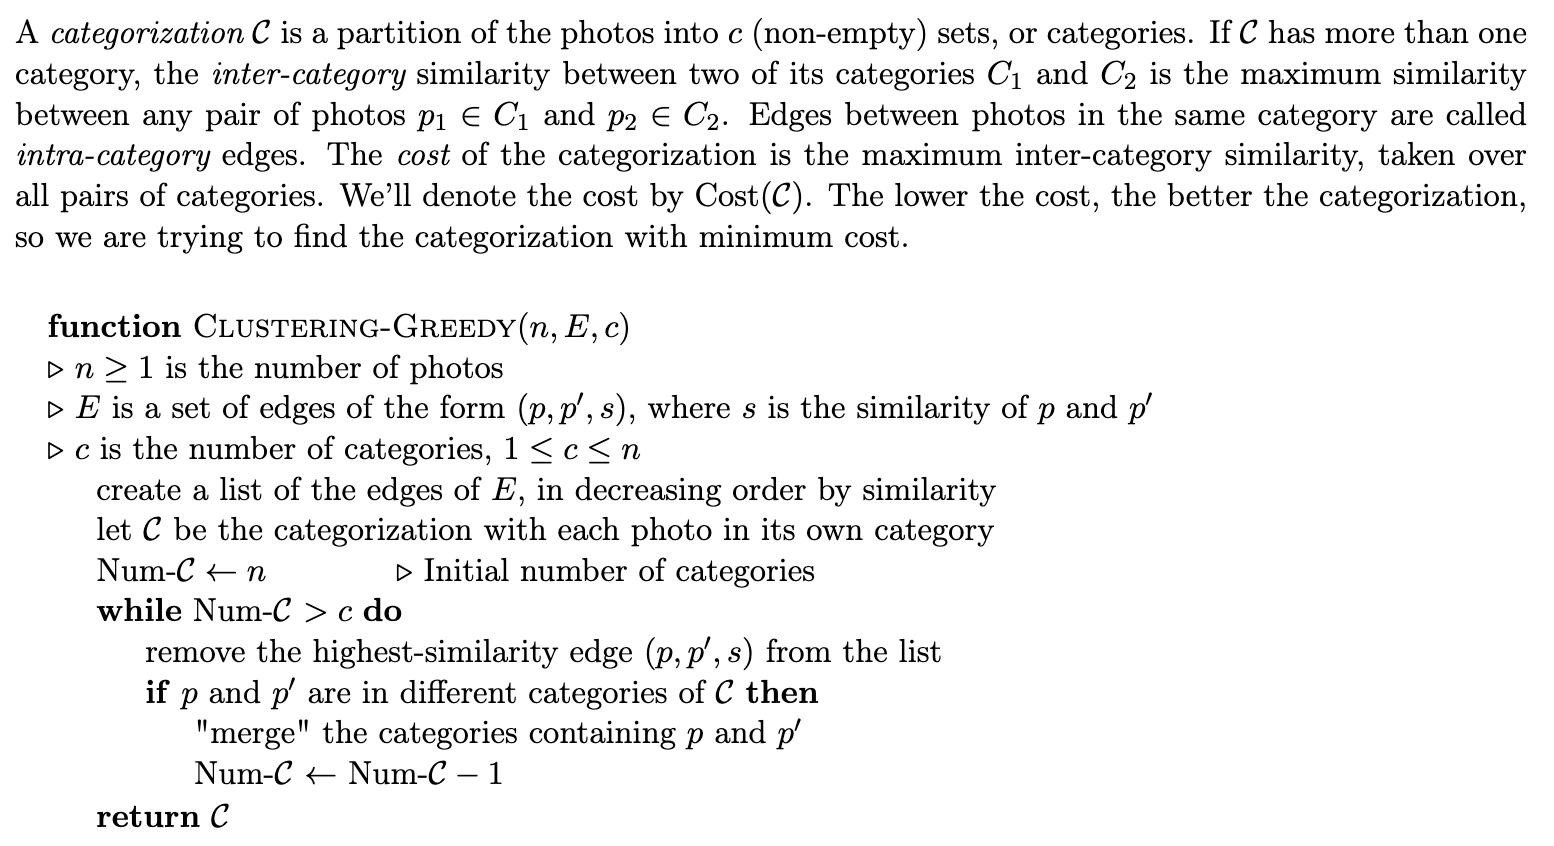
\includegraphics[width=\linewidth]{sheetimages/clustering.png}

    \hl{Knapsack with structured weights}:

    Refer to next sheet for knapsact description. Structured weights: capacity = 1, each $w_i \in \{1/16, 1/8, 1/4, 1/2\}$, unlimited supply of dummy items of each weight with value 0.

    \textbf{Solving the algorithm (GREEDY)}

    \begin{enumerate}
        \item Given an instance $I$ of problem, create a new instance $I'$.
        \item Sort the $1/16$ weights of array $W$ in decreasing order. Pair them up.
        \item Combine the weights and values of them, put into $I'$: $w_i + w_j$, $v_i + v_j$
              \begin{itemize}
                  \item $W = [1, 2]$
                  \item $V = [1/16, 1/16]$
                  \item This becomes $W=[3]$, $V=[1/8]$
              \end{itemize}
        \item Once all $1/16$ weights are eliminated, repeat for $1/8$, $1/4$, and $1/2$.
              At the end, there will be multiple $1/2$ items. Select the two items with
              the highest value. That is the solution.
    \end{enumerate}

    \textbf{Knapsack Exchange Argument}

    Use an exchange argument to prove that if an optimal solution uses $c$ items of weight $1/16$, it uses $c$ of the highest value $1/16$-weight objects.

    \begin{itemize}
        \item Imagine that Solution $S$ (subset of $\{1, 2, \ldots, n\}$) uses $c$ items with weight $1/16$,
              but NOT the $c$ highest value $1/16$-weight items.
        \item You can always swap in a higher-value $1/16$-weight item to get a better solution, so $S$ could not have
              been optimal.
        \item The same reasoning is applied for $1/8$, $1/4$, $1/2$.
        \item We have unlimited supply of dummy items, so this works, and is optimal because of
              the exchange argument approach.
    \end{itemize}

    \textbf{Proving that the optimal Knapsack Solution uses even number of weights}

    Suppose not, that you have an optimal solution that uses an odd number of items. If you add up all the weights in the solution, then the numerator has to be odd also. Since $C = 1 = 16/16$, we can always add at least one more $1/16$-weight item. This is why we need an unlimited supply of $0$-value items of $1/16$, $1/8$, \ldots, $1/2$.


    \hl{Minimizing Lateness}
    \begin{itemize}
        \item Single resource and request for $n$ requests. Each request $i$ requires time $t_i$ and has deadline $d_i$. Schedule all requests to minimize the maximum lateness:
              $
                  L = \max_i (\text{finish}_i - d_i) \quad (\text{0 if before deadline})
              $
        \item \textbf{Earliest Deadline First:} Sort jobs by their deadlines and schedule them in that order.
        \item \textbf{Proof: Exchange Argument}
              \begin{itemize}
                  \item Lemma: There exists an optimal schedule with no inversions.
                  \item If an optimal schedule $O$ has an inversion, you can swap the two jobs.
                  \item This swap does not increase the maximum lateness.
                  \item By repeatedly swapping, you convert $O$ into $G$, proving $G$ is also optimal.
              \end{itemize}
    \end{itemize}

    \hl{Optimal Caching}
    \begin{itemize}
        \item Cache of size $k$ and sequence of data item requests $d_1,\dots,d_m$. If a requested item is not in the cache, bring it in, potentially evicting another item. Goal: minimize total cache misses.
        \item \textbf{Farthest in Future:} When eviction is necessary, evict the item that will be requested farthest in the future.
        \item \textbf{Proof: Exchange Argument}
              \begin{itemize}
                  \item Lemma: Let $G$ be the schedule produced by the greedy algorithm. Let $O$ be the optimal schedule that agrees with $G$ on the first $j$ requests. Then there exists a schedule $O'$ that agrees with $G$ on the first $j+1$ requests, and incurs no more cache misses than $O$.
                  \item By repeatedly applying this lemma, $O$ can be transformed step by step into $G$ without increasing cache misses. Since $O$ is optimal, $G$ is optimal.
              \end{itemize}
    \end{itemize}

    \hl{Shortest Paths (Dijkstra's)}
    \begin{itemize}
        \item Find shortest path from a start node $s$ to all other nodes in a directed graph with non-negative edge weights $w_e \ge 0$.
        \item Maintain set $S$ of visited nodes for which the shortest path is known. Repeatedly select node $v \notin S$ that minimizes $d(u) + w_{uv}$ for some edge $(u,v)$ where $u \in S$. Add $v$ to $S$ and set $d(v) = d(u) + w_{uv}$.
        \item \textbf{Proof: Greedy Stays Ahead}
              \begin{itemize}
                  \item Lemma (Dijkstra's invariant): For every node $u \in S$, $d(u)$ is the length of the true shortest path from the start node to $u$.
                  \item Base Case: True for $S = \{s\}$, since $d(s) = 0$.
                  \item Inductive Step: Adding node $v$ via an edge. If a shorter path $P$ exists, it must cross the boundary at some edge $(x,y)$. Non-negative weights and greedy selection ensure the path via $(u,v)$ is at least as short as any path crossing the boundary.
              \end{itemize}
    \end{itemize}

    \hl{Minimum Spanning Tree}
    \begin{itemize}
        \item Given a connected graph with edge costs, find a subset of edges connecting all nodes (a tree) with minimum total cost.
        \item \textbf{Prim's:} Start with a root node. Iteratively add the cheapest edge connecting a node in the tree to a node outside.
        \item \textbf{Kruskal's:} Sort all edges by weight, iterate through them, and add only if it doesn’t create a cycle.
        \item If all edge costs are distinct, the minimum-cost edge crossing any cut $(S, V-S)$ must belong to every MST. Both algorithms implicitly select such cut-crossing edges.
    \end{itemize}

    \hl{Greedy Clustering}
    \begin{itemize}
        \item Partition photos into $c$ categories to minimize the ``cost'' (maximum similarity between any two nodes in different categories).
        \item Initially, each node is a category. Sort edges by similarity descending. Iteratively merge the two categories connected by the highest similarity edge until $c$ categories remain.
        \item Greedy choice is optimal: the cost of greedy solution $G$ satisfies $G \le$ cost of any optimal solution $O$ because greedy eliminates the highest weight inter-category edges first.
    \end{itemize}

    \hl{Night at Museum (Interval Covering)}
    \begin{itemize}
        \item Minimize guards to cover artifacts at positions $X$. Each guard covers $[pos-d, pos+d]$.
        \item Sort artifacts by position. Place guard at $x_\text{first} + d$. Remove all covered artifacts. Repeat.
        \item ``Greedy Stays Ahead'': the $i$-th greedy guard is always $\ge$ position of $i$-th guard in optimal.
    \end{itemize}

    \hl{Watch Committee}
    \begin{itemize}
        \item Select minimum number of guards so every non-selected guard overlaps with at least one selected guard.
        \item Sort shifts by start time. Maintain $S_\text{max}$ (shift with latest finish time seen so far). Iterate through shifts. If a shift starts after current covered time, select $S_\text{max}$, update covered time to $S_\text{max.finish}$, reset $S_\text{max}$.
        \item Counter-example to simple greedy: picking the shift with latest finish immediately is suboptimal (one long shift vs two disjoint shifts covering more neighbors).
    \end{itemize}

    \hl{Visa Processing}
    \begin{itemize}
        \item Schedule $n$ jobs. Job $i$ takes $e_i$ time to process (serial) and $p_i$ time for paperwork (parallel). Minimize completion time.
        \item Sort by decreasing $p_i$. Process job with longest paperwork first.
        \item \textbf{Proof: Exchange Argument}: Swapping adjacent jobs $(i,j)$ where $p_i < p_j$ reduces or maintains completion time.
    \end{itemize}

    \hl{Meet and Greed}
    \begin{itemize}
        \item Find maximum subset of people where everyone knows $\ge 4$ others in subset and does not know $\ge 4$ others outside subset.
        \item Iteratively remove any node with degree $<4$ or degree $>|S|-5$. Repeat until stable.
        \item Correctness: If a node violates the condition, it cannot be in the optimal set. Removing it is safe.
    \end{itemize}

    \section{DP}

    DP does \textbf{not help} with
    \begin{itemize}
        \item divide-and-conquer problems that partition unoverlapping spaces
        \item already dominated state costs: $T(n)=T(\lfloor n/2\rfloor)+T(\lceil n/2\rceil)+n$ (helps $T(n)=T(\lfloor n/2\rfloor)+T(\lceil n/2\rceil)+1$)
    \end{itemize}

    \hl{Steps}: (1) Recursion definition (2) Memo (Top-down) or Table (Bottom-up) (3) Extract solution

    % 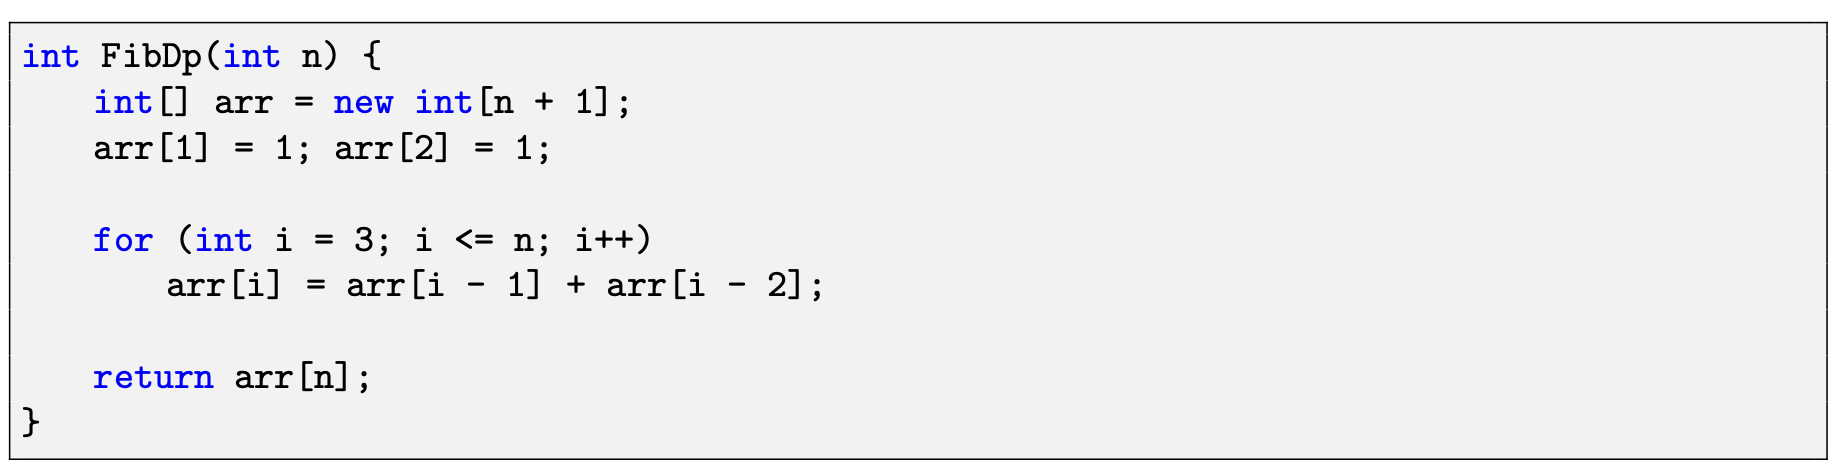
\includegraphics[width=\linewidth]{sheetimages/bottomup.png}

    % 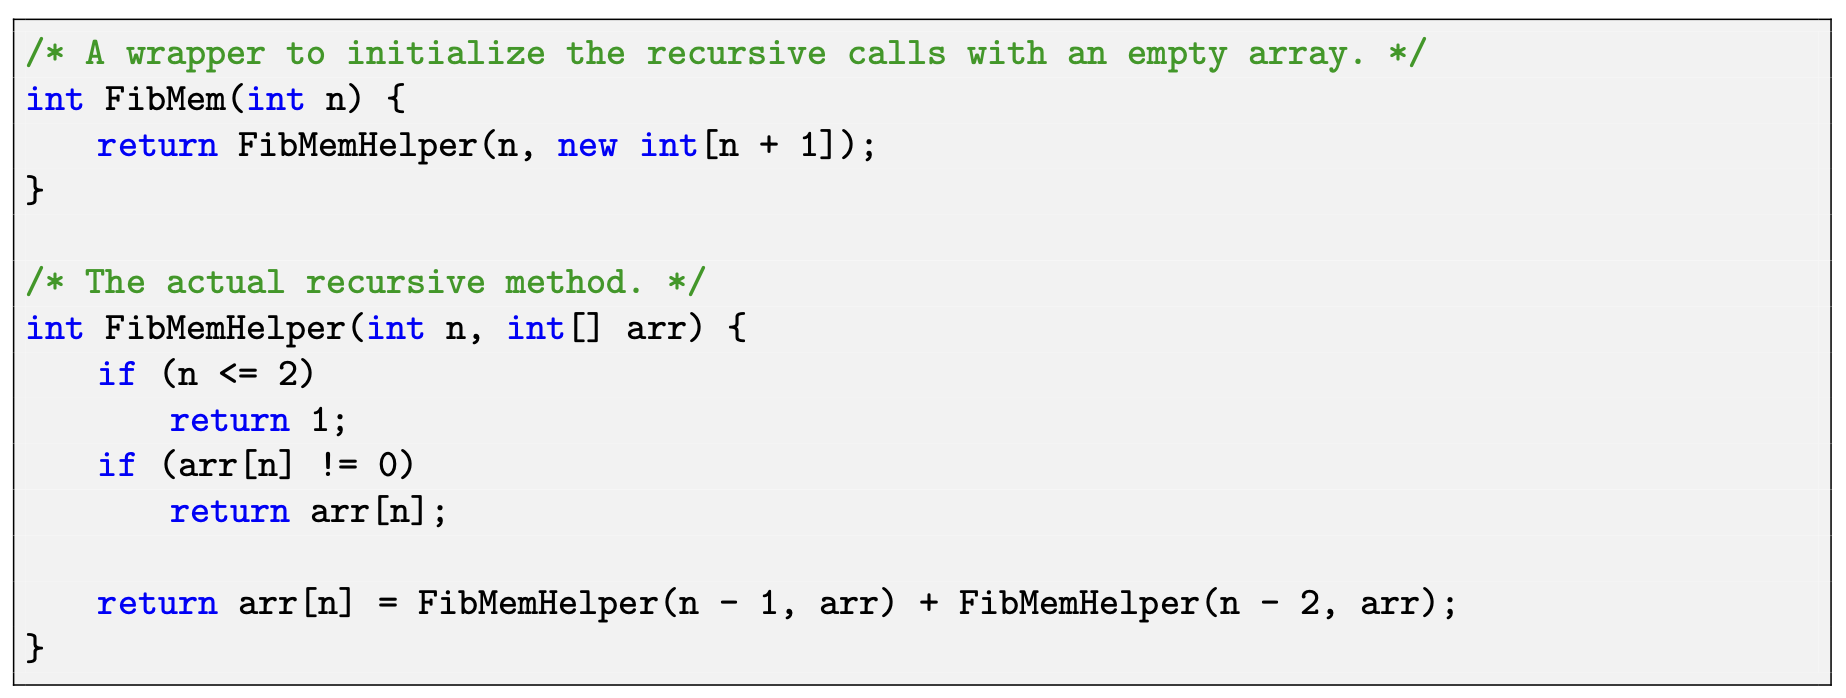
\includegraphics[width=\linewidth]{sheetimages/topdown.png}

    \hl{Coin change:}

    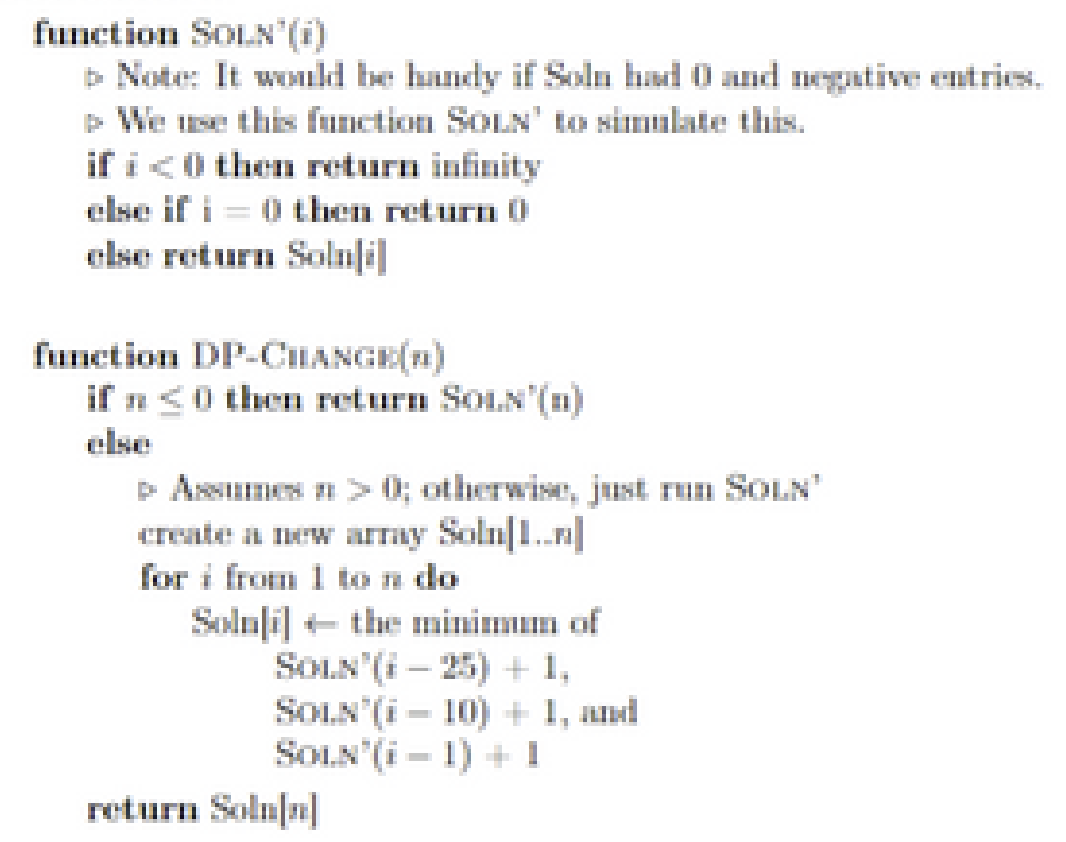
\includegraphics[width=.8\linewidth]{sheetimages/coin.png}

    % \hl{Recurrences}:

    % 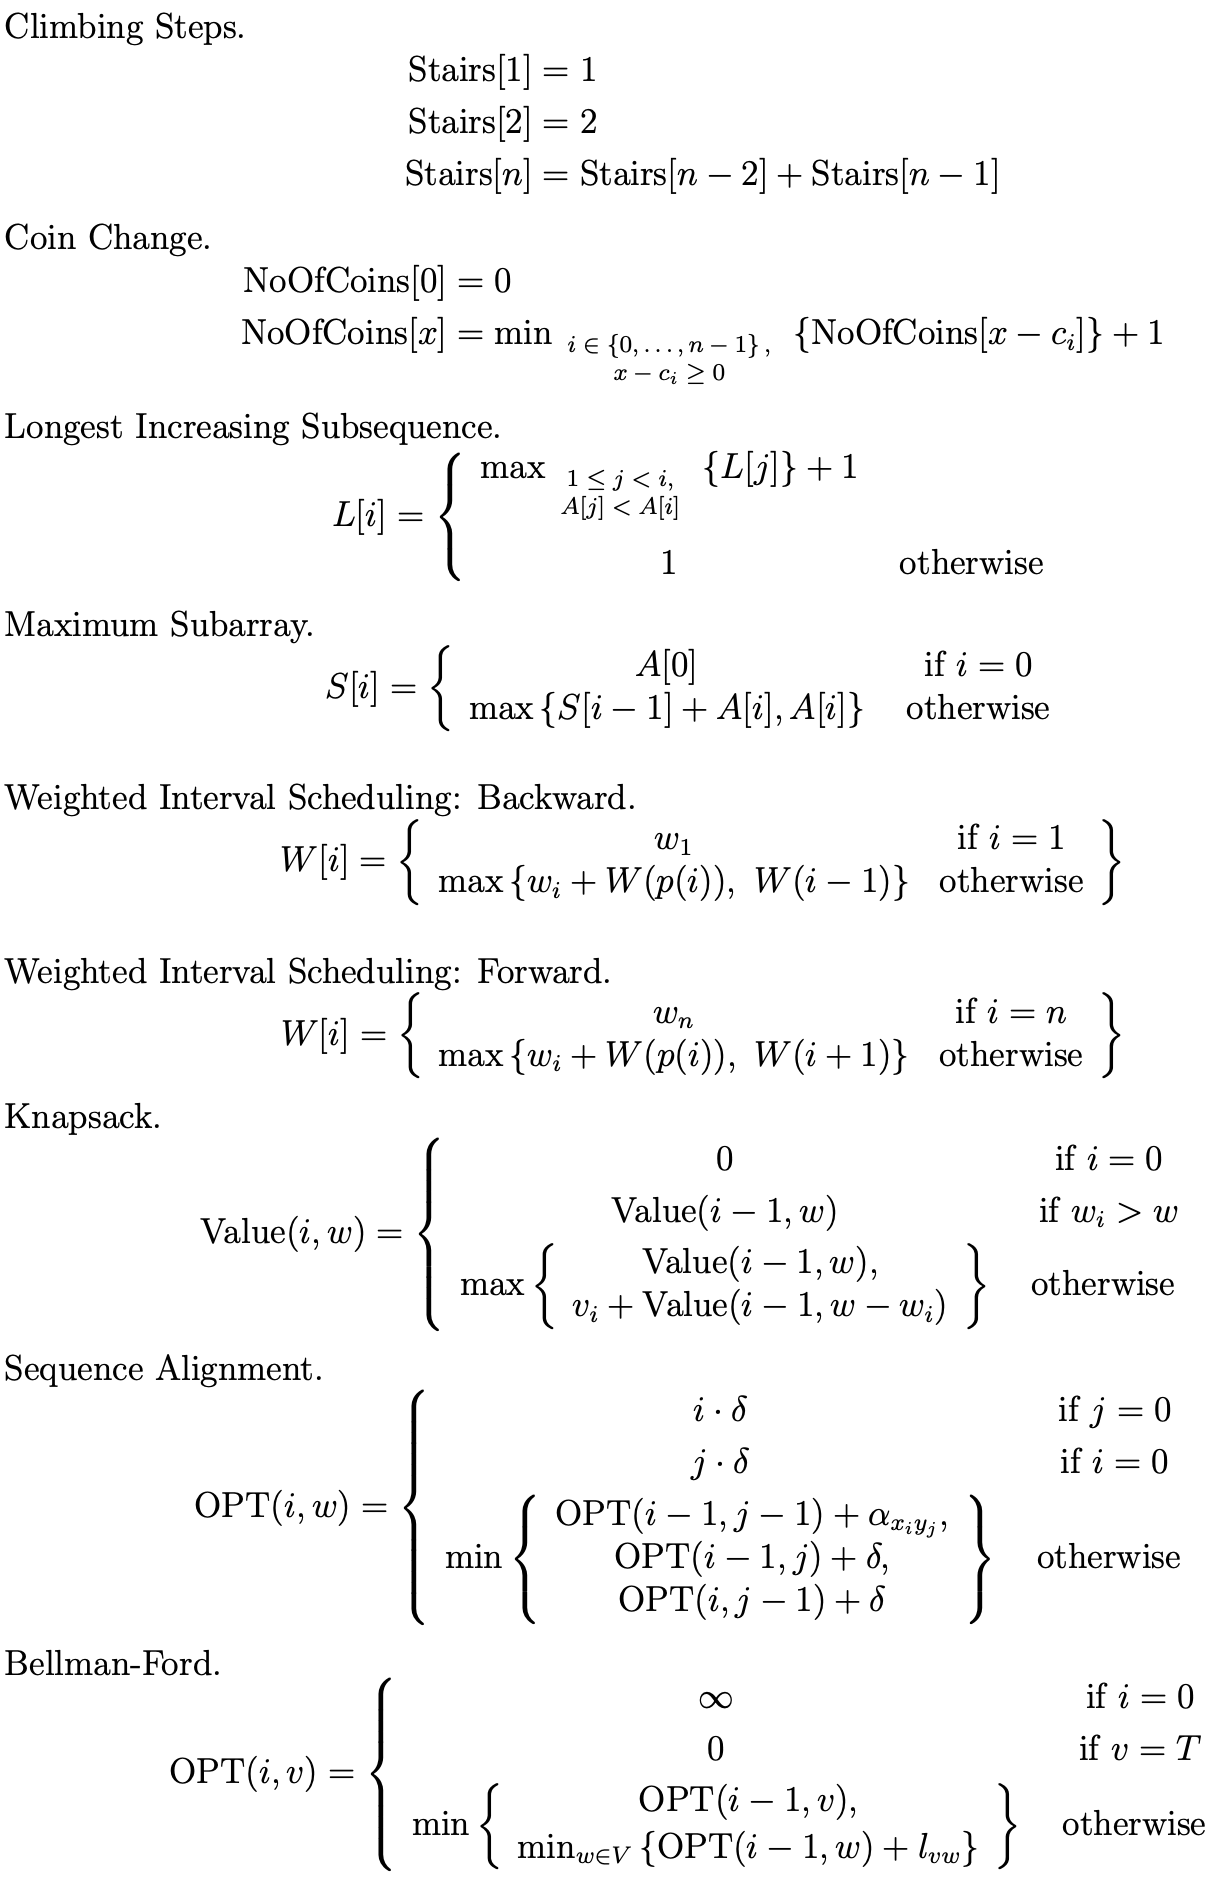
\includegraphics[width=.8\linewidth]{sheetimages/dprecurrences.png}

    \hl{Weighted node selection}:

    For an array of numbers [$v_1, v_2, \ldots, v_n$], select a subset of indices s.t.  if a node $i$ is chosen, nodes $i-1, i-2 \ldots i-v_i$ cannot be chosen. Maximize sum of chosen values.

    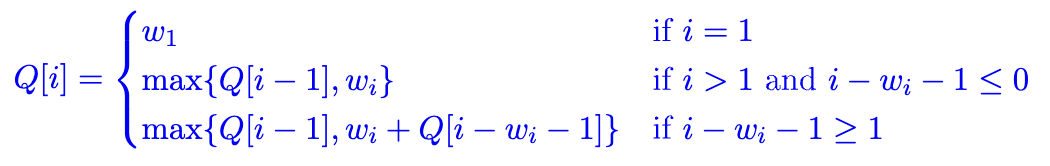
\includegraphics[width=\linewidth]{sheetimages/pathchoosing.png}

    \hl{Longest wiggling subsequence}:


    \textbf{Problem (short)}
    Given $S[1..n]$ (integers, consecutive values differ), select a longest subsequence of indices (in order) whose scariness alternates up/down/up/... or down/up/down/... . Output indices of chosen movies.

    \textbf{Greedy (naive) and counterexample}
    \begin{itemize}[noitemsep]
        \item Naive greedy: take $S_1,S_2$, then accept each next movie iff it continues alternating.
        \item Shortest counterexample: $10,20,30,25$. Greedy chooses $10,20$ (stuck); optimal is $10,30,25$.
    \end{itemize}

    \textbf{Dynamic Programming (key points)}
    \begin{itemize}[noitemsep]
        \item Subproblem parameters: $N(i,\text{up}) =$ length of longest alternating sequence \emph{ending at index $i$} where the \emph{next} step should be ``up'' (i.e. last move was down). $\text{up}\in\{\mathrm{T},\mathrm{F}\}$.
        \item Base: $N(1,\mathrm{T})=N(1,\mathrm{F})=1$.
        \item Recurrence (for $i\ge2$): \[N(i,\text{up})=\begin{cases}i&\text{if }i\leq1\\1+\max_{j=0}^{i-1}\left(N(j,\mathrm{False})\text{ if }S[i]<S[j]\right)&\text{if up}\\1+\max_{j=0}^{i-1}\left(N(j,\mathrm{True})\text{ if }S[j]<S[i]\right)&\text{otherwise}\end{cases}\]
              %   \[
              %       \begin{aligned}&N(i,up)=\begin{cases}i&\mathrm{if~}i\leq1\\1+\max_{j=0}^{i-1}\left(N(j,\mathrm{False})\mathrm{~if~}S[i]<S[j]\right)&\mathrm{if~}up\\1+\max_{j=0}^{i-1}\left(N(j,\mathrm{True})\mathrm{~if~}S[j]<S[i]\right)&\mathrm{otherwise}&\end{cases}\end{aligned}
              %   \]
              treat empty max as $0$ (so minimum is $1$).
        \item Final length: $\max(N(n,\mathrm{T}),N(n,\mathrm{F}))$ (one can show an optimal sequence can end at $n$).
        \item Store \textbf{prev} pointer for each $(i,\cdot)$ = argmax to reconstruct indices.
    \end{itemize}

    \textbf{DP pseudocode (condensed)}

    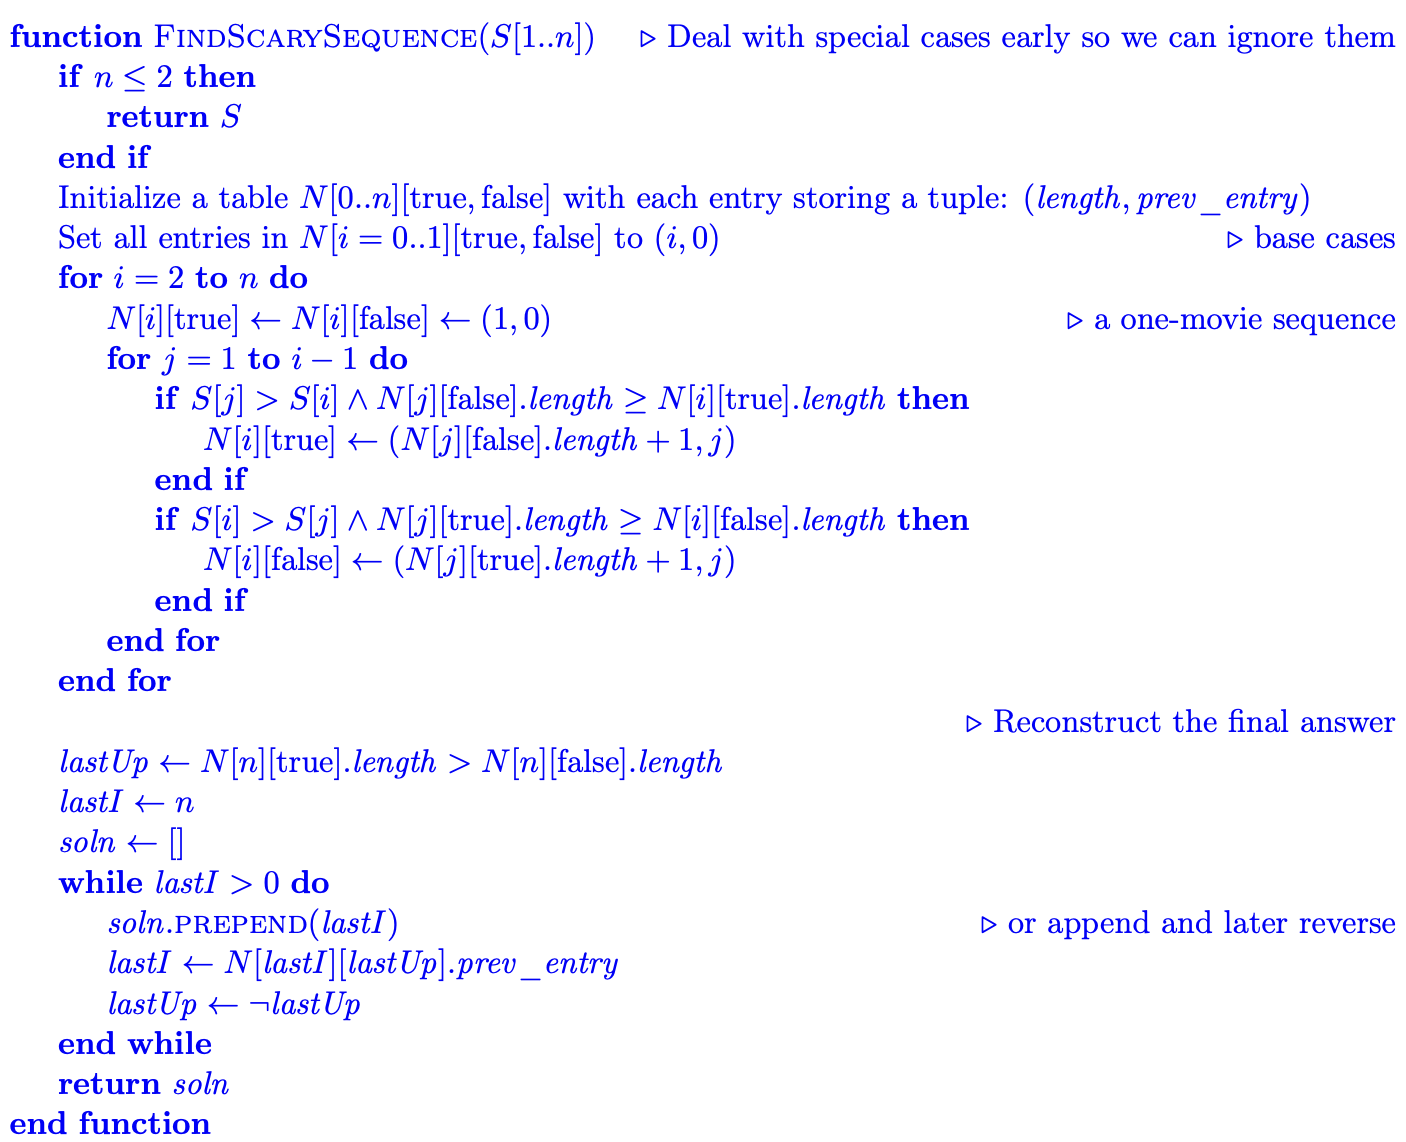
\includegraphics[width=\linewidth]{sheetimages/scary.png}

    \textbf{Complexity}
    \begin{itemize}[noitemsep]
        \item Time: $\Theta(n^2)$ (double loop).
        \item Space: $\Theta(n)$ entries $\times$ 2 states $\Rightarrow \Theta(n)$ (plus prev pointers).
    \end{itemize}

    \textbf{Linear-time greedy (optimal) — sketch}
    \begin{itemize}[noitemsep]
        \item Maintain candidate list \texttt{Cands} of chosen values (indices or values).
        \item For each $S[i]$:
              \begin{itemize}[noitemsep]
                  \item If $S[i]$ continues the same direction as last two \texttt{Cands} and extends that direction farther, replace the last candidate by $S[i]$.
                  \item Else append $S[i]$ (it flips direction).
              \end{itemize}
        \item Runs in $O(n)$ and yields an optimal alternating subsequence when consecutive values are distinct.
    \end{itemize}

    \hl{Example memo DP}:

    $D(i,n)=\begin{cases}0&i<1\lor n<i\\D(i-1,n-1)D(i-2,n-i)+f(i,n)&\text{ otherwise }\end{cases}$

    \begin{verbatim}
memo = {}   # keys are tuples (i,n)

def D(i, n):
    # base cases
    if i < 1 or n < i:
        return 0
    if (i, n) in memo:
        return memo[(i, n)]
    # compute subresults (memoization prevents re-computation)
    a = D(i-1, n-1)
    b = D(i-2, n-i)
    val = a * b + f(i, n)   # assume arithmetic of f(i,n) is included in cost
    memo[(i, n)] = val
    return val
    \end{verbatim}

    \hl{Example bottom up DP}:

    Solve for all $b \in [0,...,n-1]$ and all $v \in V$:

    $P(b,v)=\min_{(u,v)\in E}\{P(b-1,u)+p(u,v)\}$

    \begin{verbatim}
P[b][s] ← 0 for all b in [0,...,n-1] 
P[0][v] ← ∞ for all v ̸= s 
For b=1, ... ,n-1: 
    For each v in V-s: 
        P[b][v] = ← ∞ 
        For each (u,v) in E: 
            If P[b-1][u] +p((u,v)) < P[b][v]: 
                P[b][v] ← P[b-1][u] + p(u,v)
    \end{verbatim}

    \hl{Weighted Interval Scheduling Problem}

    Each interval $i$ has a start time $s_i$, finish time $f_i$, and weight (value) $w_i$.
    The goal is to choose a set of mutually non-overlapping intervals with maximum total
    weight.

    \textbf{Preprocessing}

    Sort intervals by increasing finish time:
    $
        f_1 \le f_2 \le \cdots \le f_n.
    $.
    For each interval $i$, compute:
    $
        p(i) = \max \{ j < i \mid f_j \le s_i \},
    $
    the index of the rightmost interval that is compatible with $i$ (or $0$ if none).

    \textbf{Dynamic Programming Recurrence}

    Let $M(i)$ be the maximum total weight using intervals $\{1,\dots,i\}$.
    Then
    \[
        M(i) =
        \begin{cases}
            0,                                         & i = 0,   \\
            \max\bigl( w_i + M(p(i)),\; M(i-1) \bigr), & i \ge 1.
        \end{cases}
    \]

    The optimal value is $M(n)$.

    \textbf{DP Algorithm (Bottom-Up)}
    \begin{verbatim}
Sort intervals by increasing finish time
Compute p(i) for all i

M[0] = 0
for i = 1 to n:
    M[i] = max( w[i] + M[p(i)],   M[i-1] )
return M[n]
\end{verbatim}

    \textbf{Constructing the Optimal Solution}
    \begin{verbatim}
function FindSolution(i):
    if i == 0: return empty set
    if w[i] + M[p(i)] >= M[i-1]:
        return {i} ∪ FindSolution(p(i))
    else:
        return FindSolution(i-1)
\end{verbatim}

    \textbf{Correctness (Brief Outline)}

    Any optimal solution for intervals $\{1,\dots,i\}$ either:
    \begin{enumerate}
        \item includes interval $i$ (thus must include an optimal solution for $p(i)$), or
        \item excludes $i$ (thus must include an optimal solution for $i-1$).
    \end{enumerate}
    These two cases yield the recurrence.

    Using induction on $i$, the DP recurrence computes the optimal value for all prefixes
    of the interval list. Hence $M(n)$ is optimal.

    \hl{Knapsack problem}:

    You find yourself with a chest full of valuable items. However, you only brought a knapsack of capacity $W$ pounds. The chest has $n$ items, where item $i$ weighs $w_i$ pounds and has value $v_i$ dollars. You must choose which items to take to maximize the total value.

    \textbf{1. Recurrence Relation}

    Let $V(i, w)$ be the maximum value obtainable by packing items from $\{1, \ldots, i\}$ with total weight $\leq w$.

    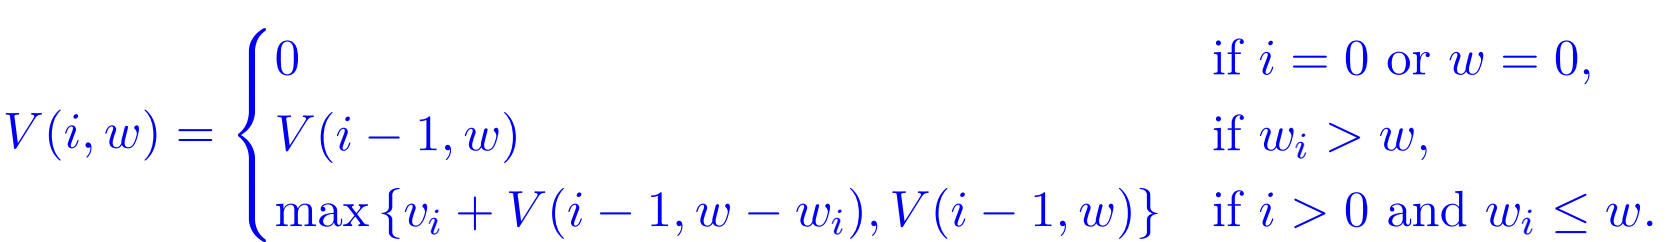
\includegraphics[width=\linewidth]{sheetimages/knapsack.png}

    \textbf{2. Iterative DP Algorithm}

    \begin{verbatim}
procedure Knapsack-Iterative(n, W)
    Let V be a 2D array of size (n+1) × (W+1)
    for i ← 0 to n do
        for w ← 0 to W do
            if i = 0 or w = 0 then
                V[i][w] ← 0
            else if w_i > w then
                V[i][w] ← V[i-1][w]
            else
                V[i][w] ← max{V[i-1][w], v_i + V[i-1][w-w_i]}
            end if
        end for
    end for
    return V[n][W]
end procedure
    \end{verbatim}

    \textbf{3. Reconstruction Algorithm}

    \begin{verbatim}
procedure Knapsack-Reconstruct(V, n, W)
    Let S be an array of at most n items
    w ← W
    i ← n
    while i > 0 do
        if V[i][w] > V[i-1][w] then
            S[i] ← (v_i, w_i)    ⊲ item i is included
            w ← w - w_i
        end if
        i ← i - 1
    end while
    return S
end procedure
    \end{verbatim}

    \hl{Segmented Least Squares}
    \begin{itemize}
        \item Given $n$ points, fit a sequence of lines to them to minimize the sum of squared errors ($E$), plus a penalty $C$ for each line used.
        \item Subproblem: $\text{OPT}(i) =$ minimum cost for points $p_1, \dots, p_i$.
        \item The last segment in the optimal solution must cover points $p_j, \dots, p_i$, for some $1 \le j \le i$.
        \item Recurrence:
              $
                  \text{OPT}(i) = \min_{1 \le j \le i} (E_{i,j} + C + \text{OPT}(j-1))
              $
    \end{itemize}

    \hl{Knapsack Problem}
    \begin{itemize}
        \item You have $n$ items, each with weight $w_i$ and value $v_i$. Max capacity $W$. Maximize total value.
        \item Subproblem: $\text{OPT}(i,w) =$ max value using a subset of the first $i$ items with weight limit $w$.
        \item Recurrence:
              $
                  \text{OPT}(i,w) = \max \begin{cases}
                      \text{OPT}(i-1,w)           & \text{skip item}                \\
                      v_i + \text{OPT}(i-1,w-w_i) & \text{take item, if } w \ge w_i
                  \end{cases}
              $
    \end{itemize}

    \hl{Sequence Alignment (Edit Distance)}
    \begin{itemize}
        \item Find the cost to transform string $X$ ($n$ chars) into $Y$ ($m$ chars). Costs: $\delta$ for a gap, $\alpha_{pq}$ for matching char $p$ with $q$.
        \item Subproblem: $\text{OPT}(i,j)$ is the min cost to align prefixes $X[1 \dots i]$ and $Y[1 \dots j]$.
        \item Recurrence:
              $
                  \text{OPT}(i,j) = \min \begin{cases}
                      \alpha_{x_i,y_j} + \text{OPT}(i-1,j-1) & \text{match/mismatch}                    \\
                      \delta + \text{OPT}(i-1,j)             & \text{gap in } Y / \text{delete from } X \\
                      \delta + \text{OPT}(i,j-1)             & \text{gap in } X / \text{delete from } Y
                  \end{cases}
              $
    \end{itemize}

    \hl{Longest Common Subsequence (LCS)}
    \begin{itemize}
        \item Find the longest string $S$ whose characters appear in order in two input strings $A$ and $B$.
        \item Recurrence:
              $
                  \text{LLCS}(A[1..n], B[1..m]) =
                  \begin{cases}
                      1 + \text{LLCS}(A[1..n-1], B[1..m-1])                    & A[n] = B[m]      \\
                      \max(\text{LLCS}(A[1..n-1],B), \text{LLCS}(A,B[1..m-1])) & \text{otherwise}
                  \end{cases}
              $
        \item Memoization: Top-down recursion storing results in a table initialized to $-1$.
        \item Iterative DP: Bottom-up table filling. Time and space complexity $O(nm)$. Space can be optimized to $O(n)$ by storing only previous columns.
    \end{itemize}

    \hl{Making Change}
    \begin{itemize}
        \item Minimize the number of coins needed to make change for amount $n$ given denominations.
        \item Greedy algorithms fail for certain currency sets.
        \item Recurrence:
              $
                  C(n) = 1 + \min \{ C(n-v_1), C(n-v_2), \dots, C(n-v_k) \}
              $
        \item Performance: Brute force is exponential; DP/memoization reduces to $O(n)$.
    \end{itemize}

    \hl{Lighting Beacons}
    \begin{itemize}
        \item Place beacons on a chain of hills from source (1) to target ($n$), max distance $100$ km, maximize probability of signal (product of individual link probabilities $P(i,j)$).
        \item Recurrence:
              $
                  \text{OPT}(j) = \max_{i<j, D(j)-D(i)\le 100} \{\text{OPT}(i) \times P(i,j)\}, \quad \text{OPT}(1) = 1
              $
        \item Complexity: $O(n^2)$ if checking all predecessors, $O(n)$ if bounded by constant number of predecessors.
    \end{itemize}

    \hl{Halloween Houses}
    \begin{itemize}
        \item Maximize total artistic merit of selected houses. Constraint: If house $i$ is “Loud”, cannot select $i-1$.
        \item If $H[i]$ is Loud:
              $
                  M(i) = \max(M(i-1), H[i].\text{merit} + M(i-2))
              $
        \item If $H[i]$ is Normal:
              $
                  M(i) = H[i].\text{merit} + M(i-1)
              $
        \item Time $O(n)$, space $O(1)$.
    \end{itemize}

    \hl{Scary Scheduling}
    \begin{itemize}
        \item Find the longest subsequence of movie ratings that alternates between increasing and decreasing.
        \item Recurrence:
              $
                  \begin{aligned}
                      N(i,\text{true})  & = 1 + \max_{j<i, S[j]<S[i]} \{N(j,\text{false})\} \\
                      N(i,\text{false}) & = 1 + \max_{j<i, S[j]>S[i]} \{N(j,\text{true})\}
                  \end{aligned}
              $
        \item Time $O(n^2)$, space $O(n^2)$ (or $O(n)$ optimized).
    \end{itemize}

    \hl{Typesetting (Line Breaking)}
    \begin{itemize}
        \item Break words into lines to minimize total penalty $(W-\text{width}(\text{line}_i))^2$.
        \item Recurrence:
              $
                  L_{\min}(i) = \min_{j<i} \{ L_{\min}(j) + (W - \text{width}(\text{words}[j+1..i]))^2 \}
              $
        \item Complexity: $O(n^2)$ or $O(nW)$ depending on implementation.
    \end{itemize}

    \hl{Signal Interleaving}
    \begin{itemize}
        \item Determine if string $s$ is an interleaving of repetitions of strings $x$ and $y$.
        \item Recurrence:
              $\begin{aligned}&I(i,j)=(s[i+j]==x[i\pmod{|x|})]\wedge I(i-1,j))\\&\vee(s[i+j]==y[j\pmod{|y|})]\wedge I(i,j-1))\end{aligned}$
        \item Complexity: $\Theta(|s|^2)$.
    \end{itemize}


    \section{Divide and Conquer}

    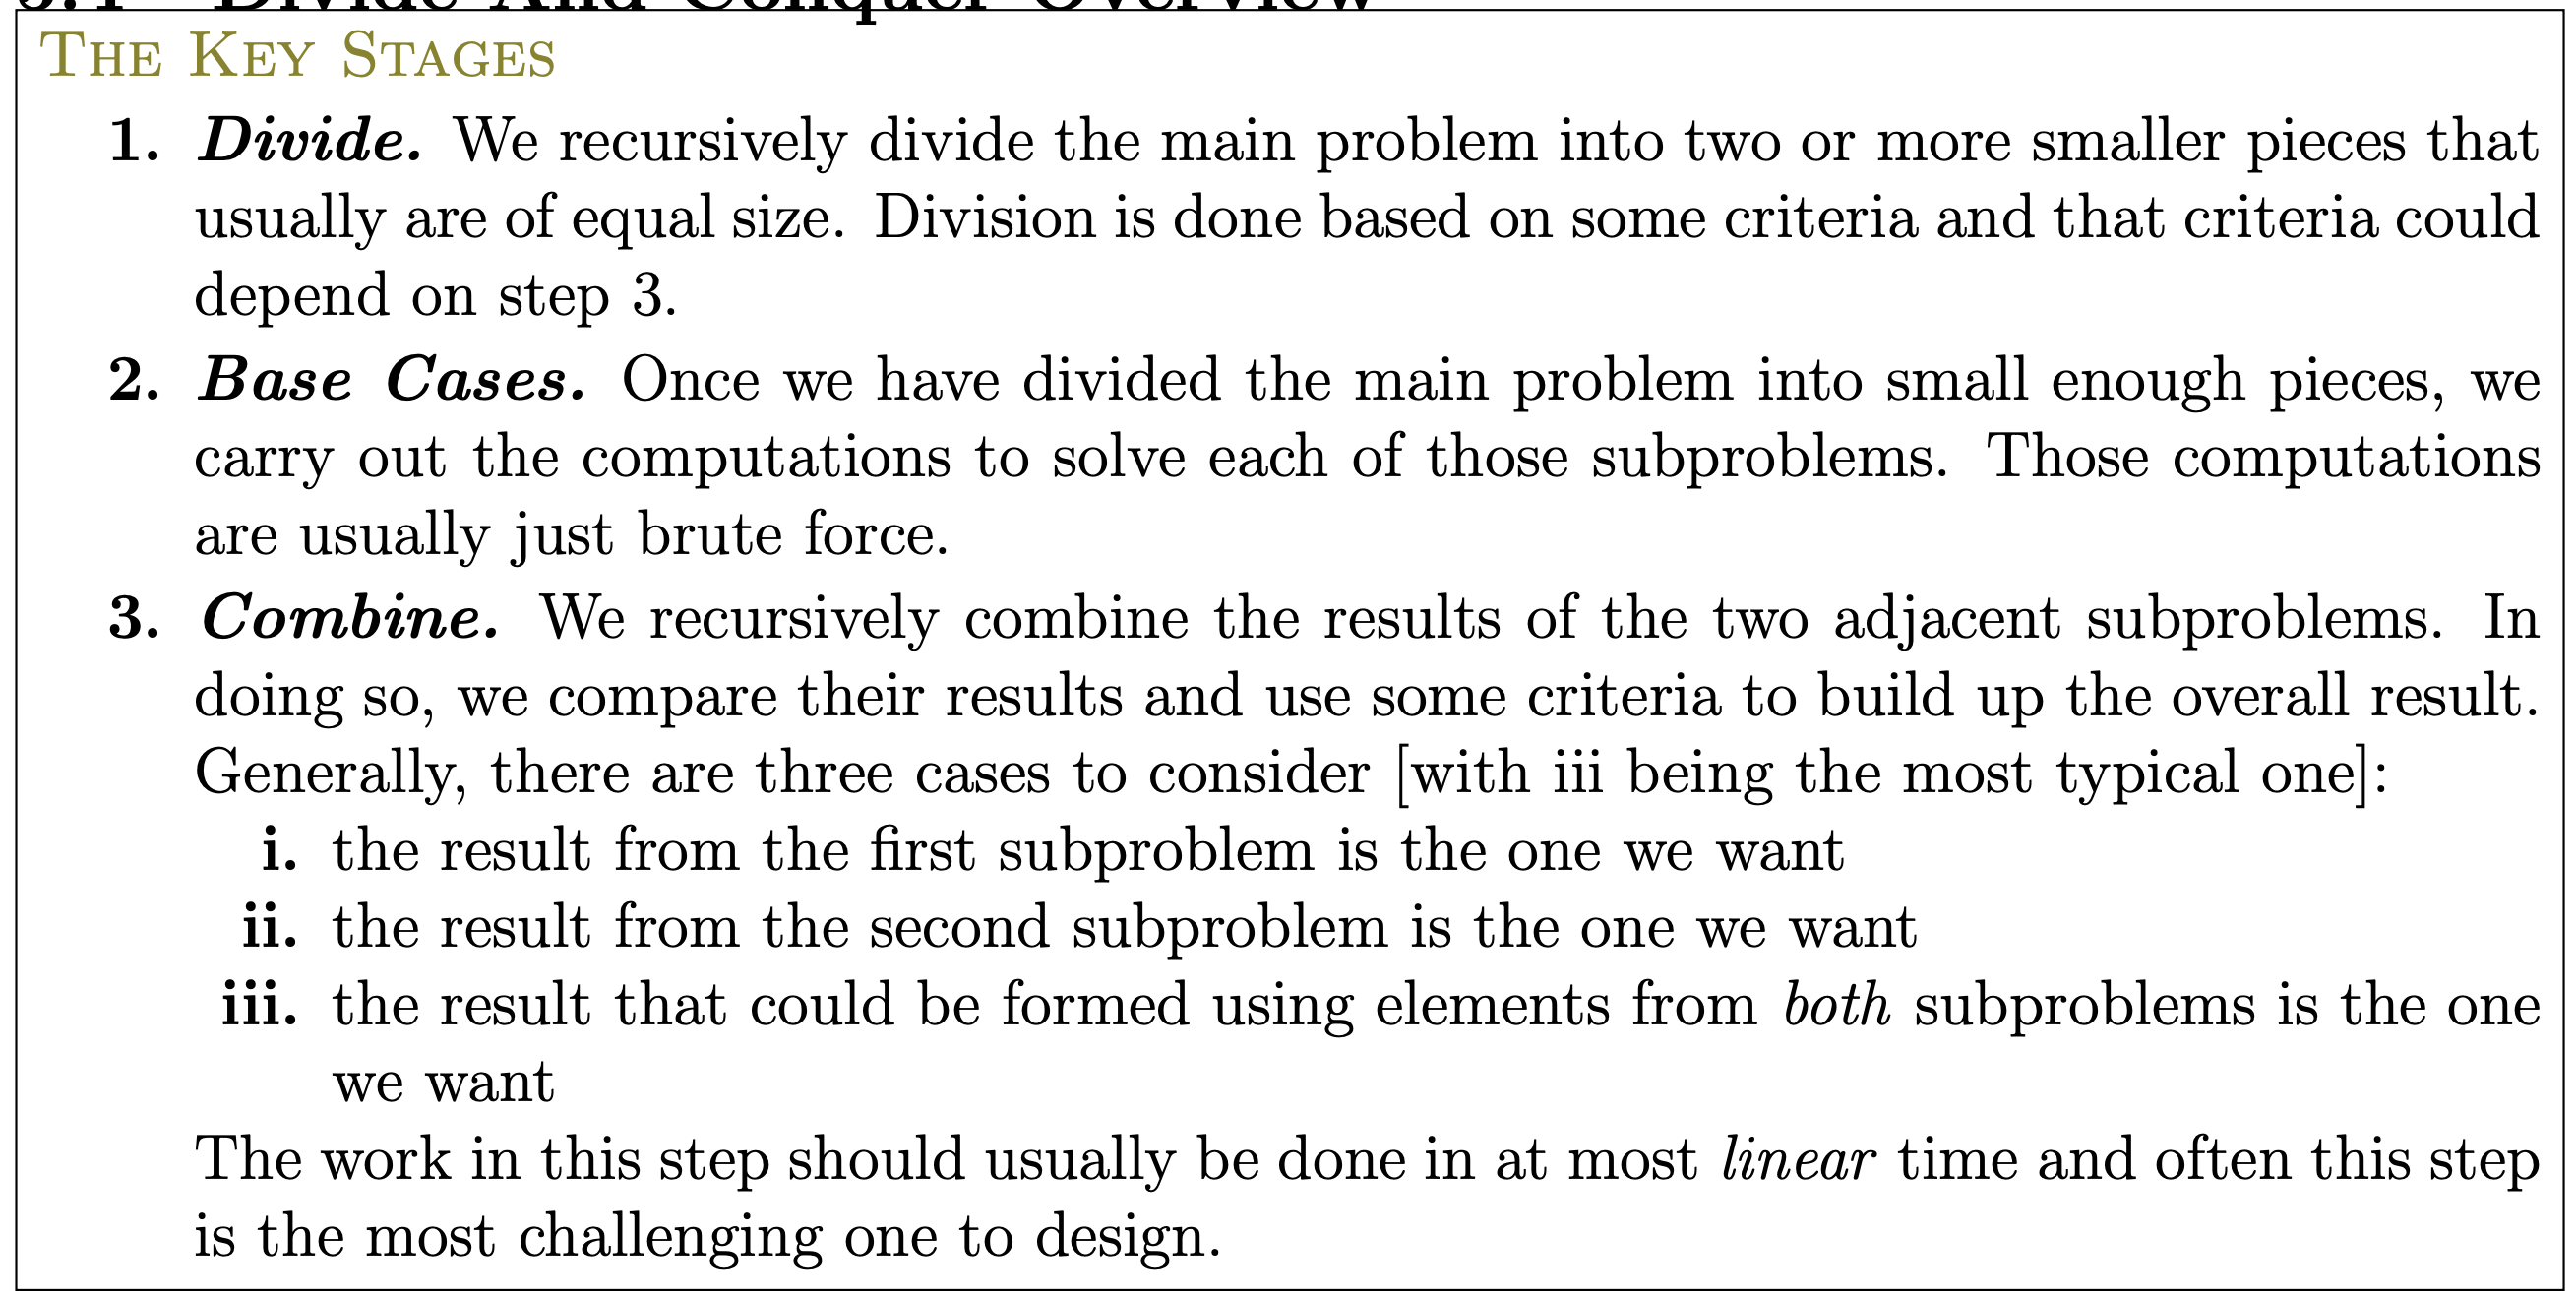
\includegraphics[width=\linewidth]{sheetimages/dnqstages.png}

    Each level work
    \begin{itemize}
        \item $cn \to T(n) \in O(n \log n)$
        \item $c(\frac{p}{q})^i n^k \to T(n) \in O(n^k), p < q$
    \end{itemize}

    \hl{Each level work factor increasing} ($p > q$): $T(n) = 3T(\frac{n}{2}) + cn$:

    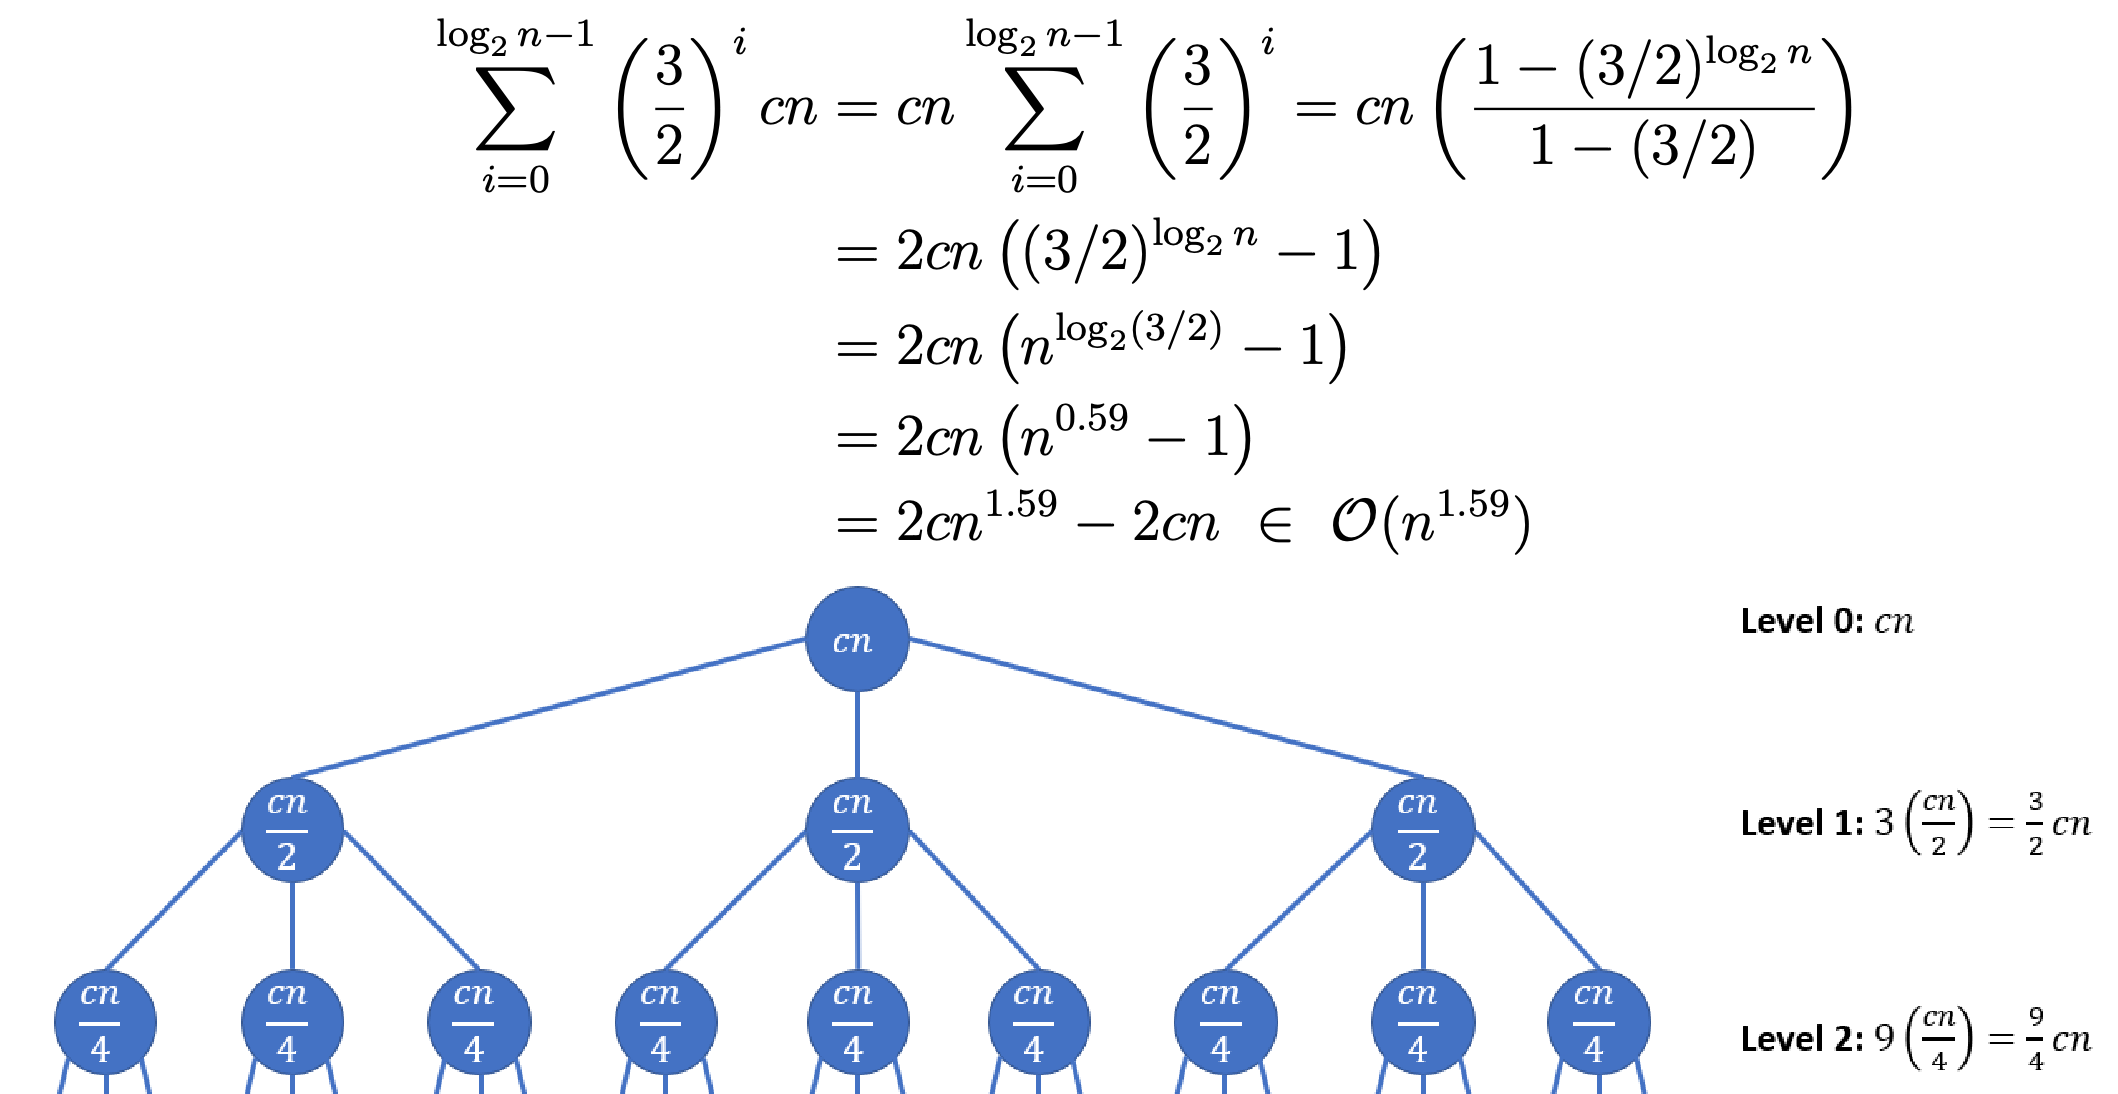
\includegraphics[width=\linewidth]{sheetimages/tree1.png}

    \hl{Each level work factor decreasing} ($p < q$):

    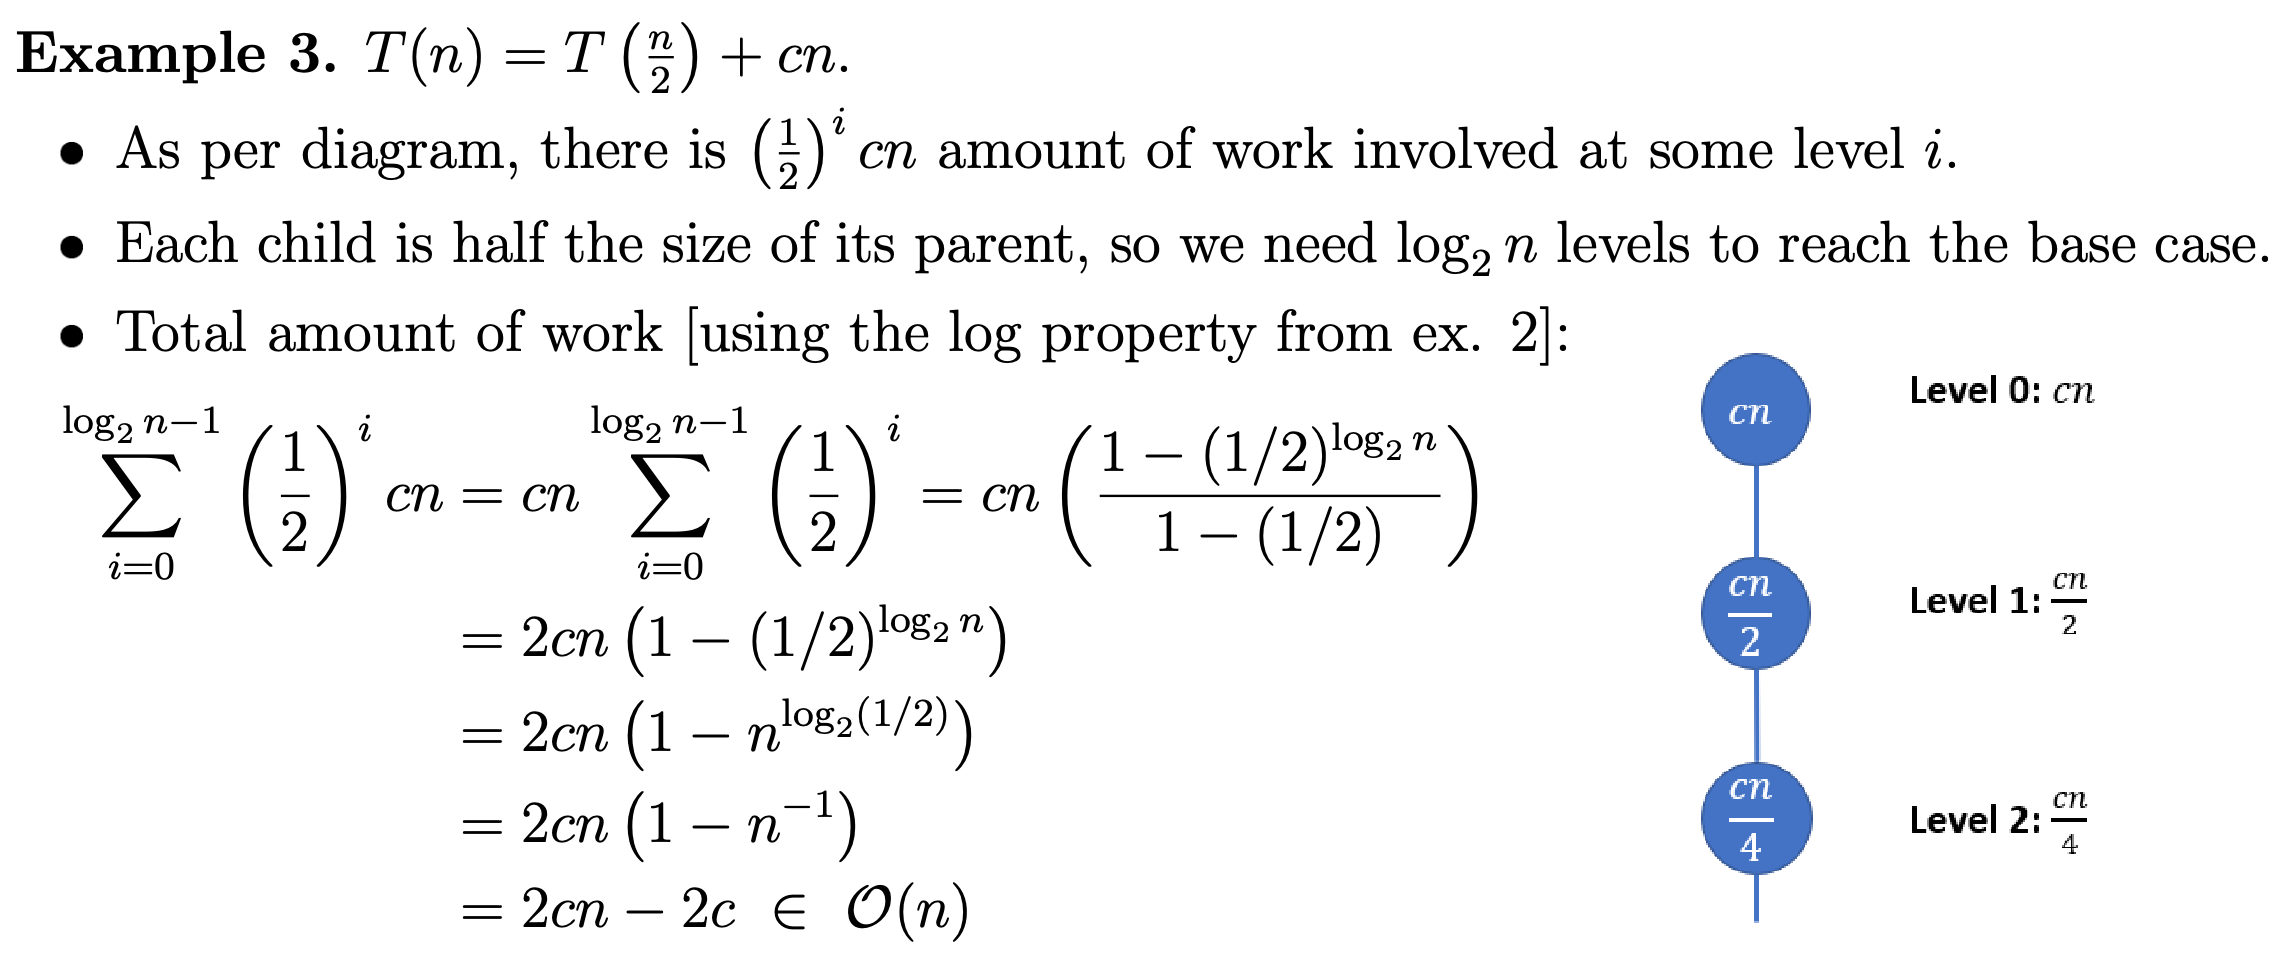
\includegraphics[width=\linewidth]{sheetimages/tree2.png}

    \hl{Each level work factor same} ($p/q = 1$):

    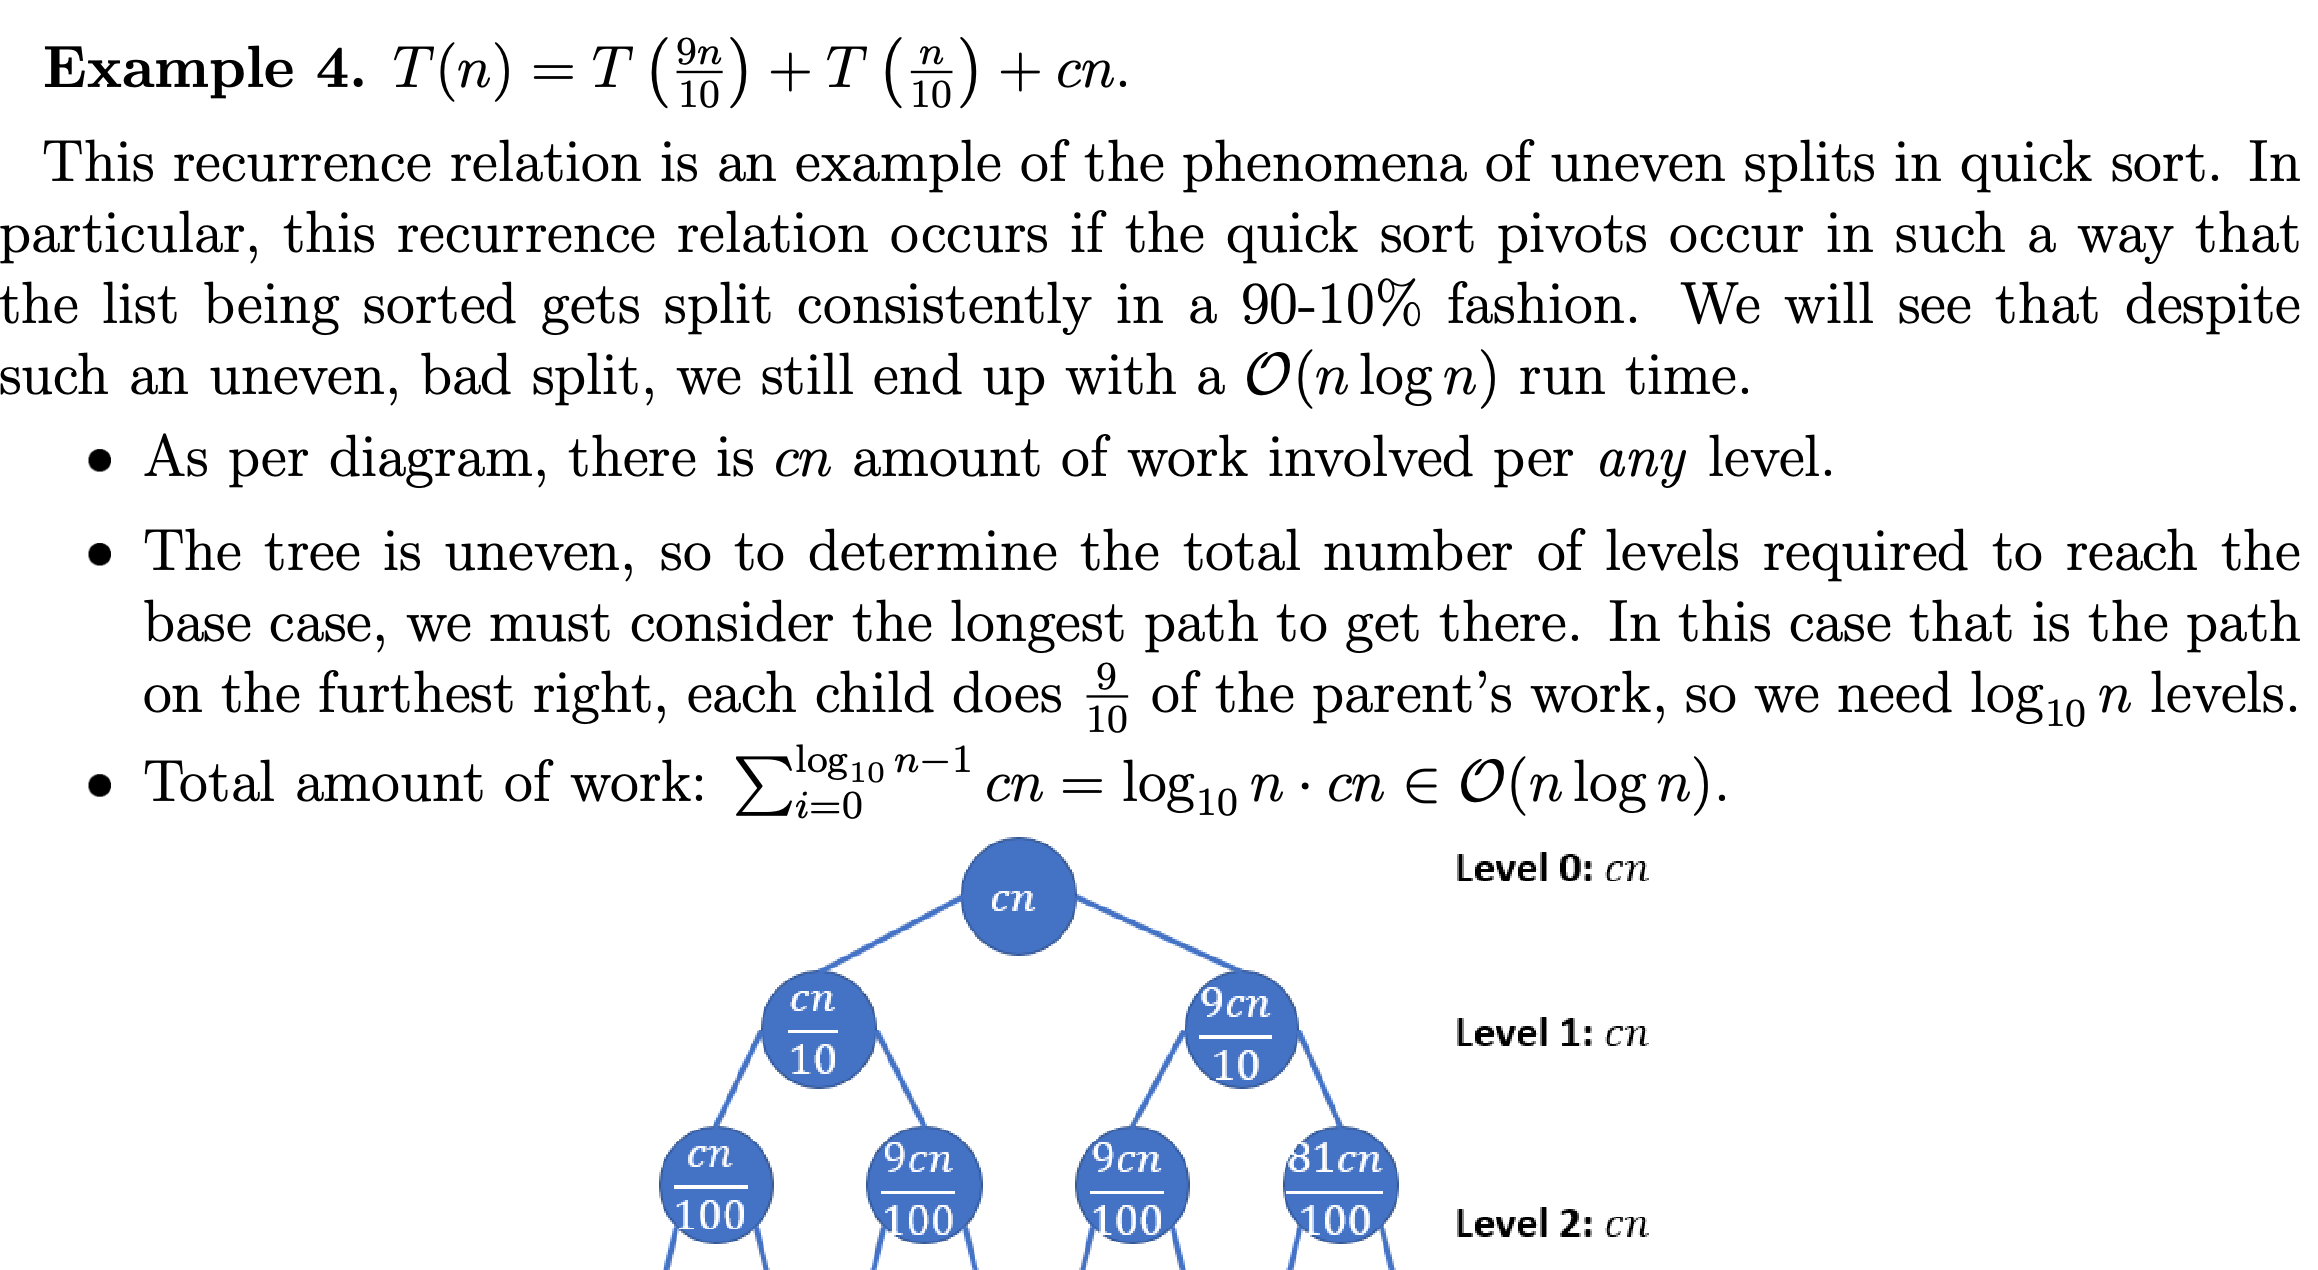
\includegraphics[width=\linewidth]{sheetimages/tree3.png}

    \hl{Deterministic select}

    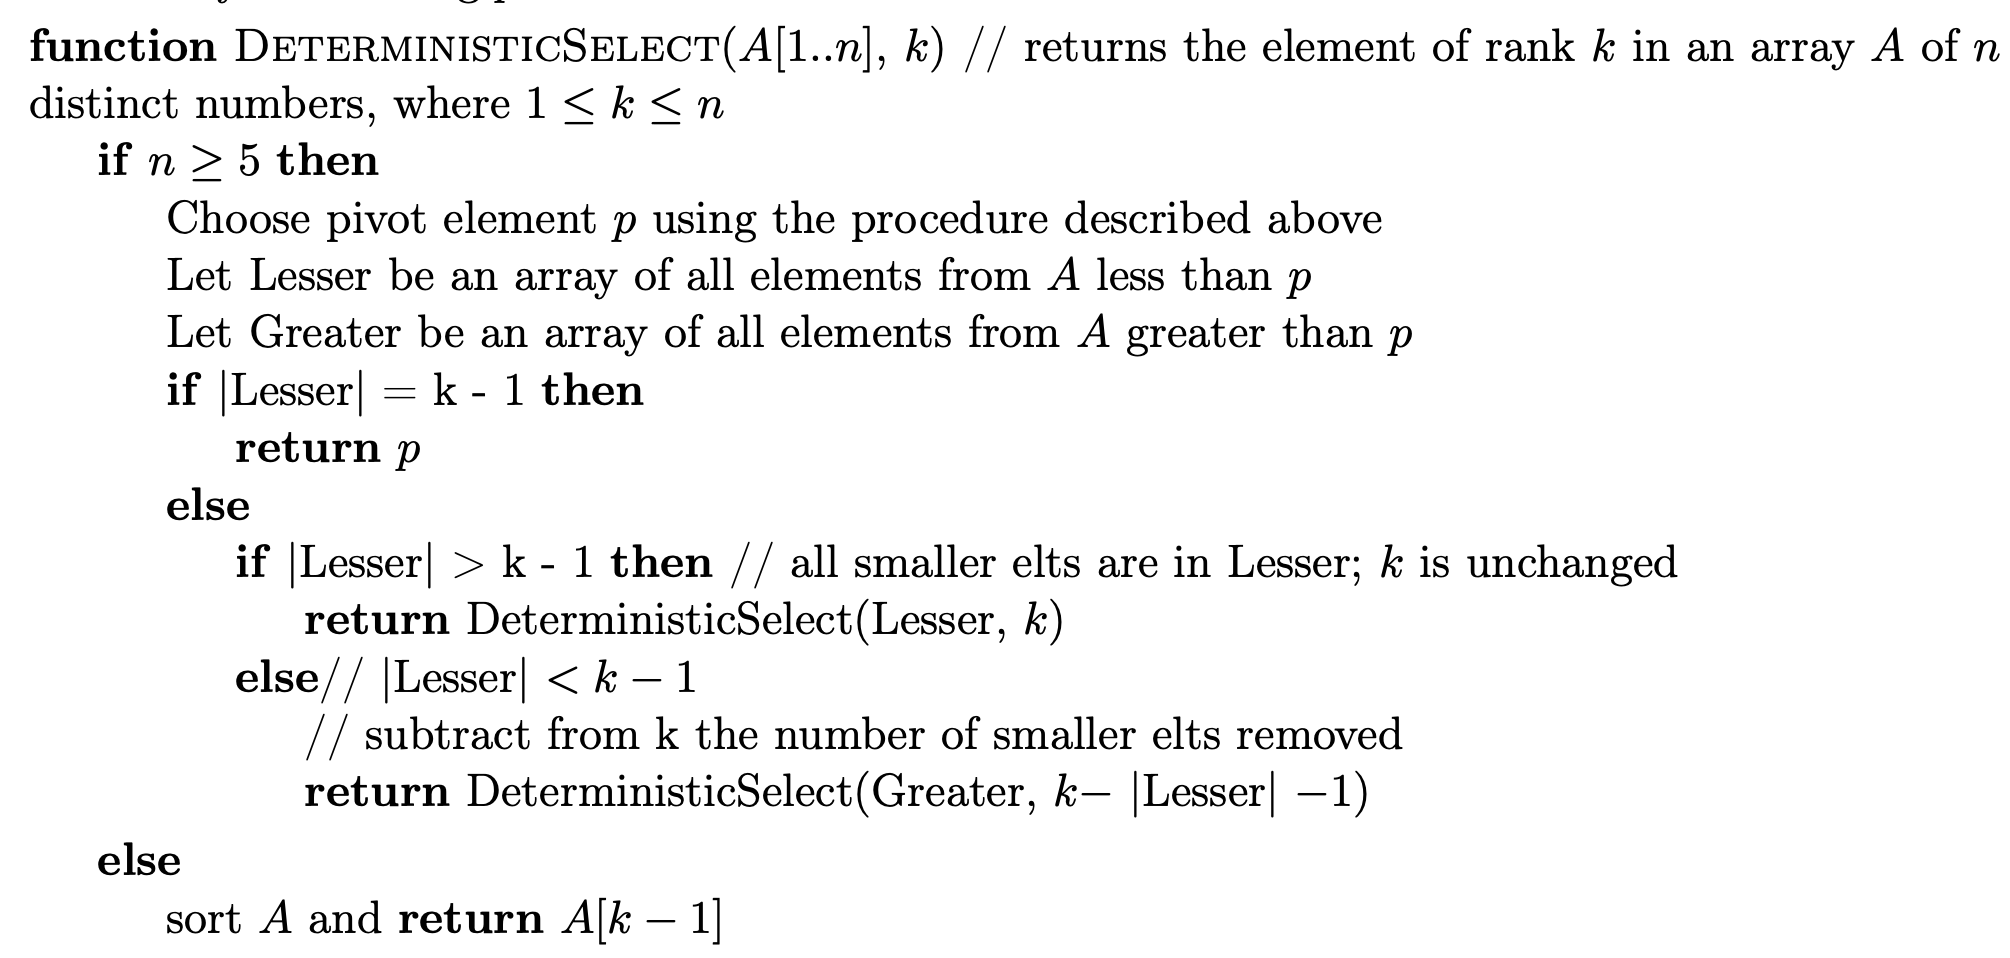
\includegraphics[width=\linewidth]{sheetimages/deterministic.png}

    The value $m$ is the median of $\lfloor n/5 \rfloor$ group medians, and so it is the $\lceil \lfloor n/5 \rfloor / 2 \rceil$ smallest of them. There are $\lfloor n/5 \rfloor - \lceil \lfloor n/5 \rfloor / 2 \rceil = \lfloor \lfloor n/5 \rfloor / 2 \rfloor$ groups with medians larger than $m$, each of which contains 3 elements larger than $m$ (the largest two, and their median). The group that contains $m$ also has two elements larger than it. So there are at least $3(\lfloor \lfloor n/5 \rfloor / 2 \rfloor) + 2$ elements larger than $m$.

    \[T(n)\leq\begin{cases}T(\lfloor n/5\rfloor)+T(7n/10+2)+cn&\text{if }n\geq5.\\\Theta(1)&\text{if }n\leq4.\end{cases}\]

    \hl{Quickselect}

    $T_{QS}(n)=\begin{cases}1&\text{if }n=0\text{ or }n=1\\T_{QS}(3n/4)+cn&\text{otherwise}\end{cases}$

    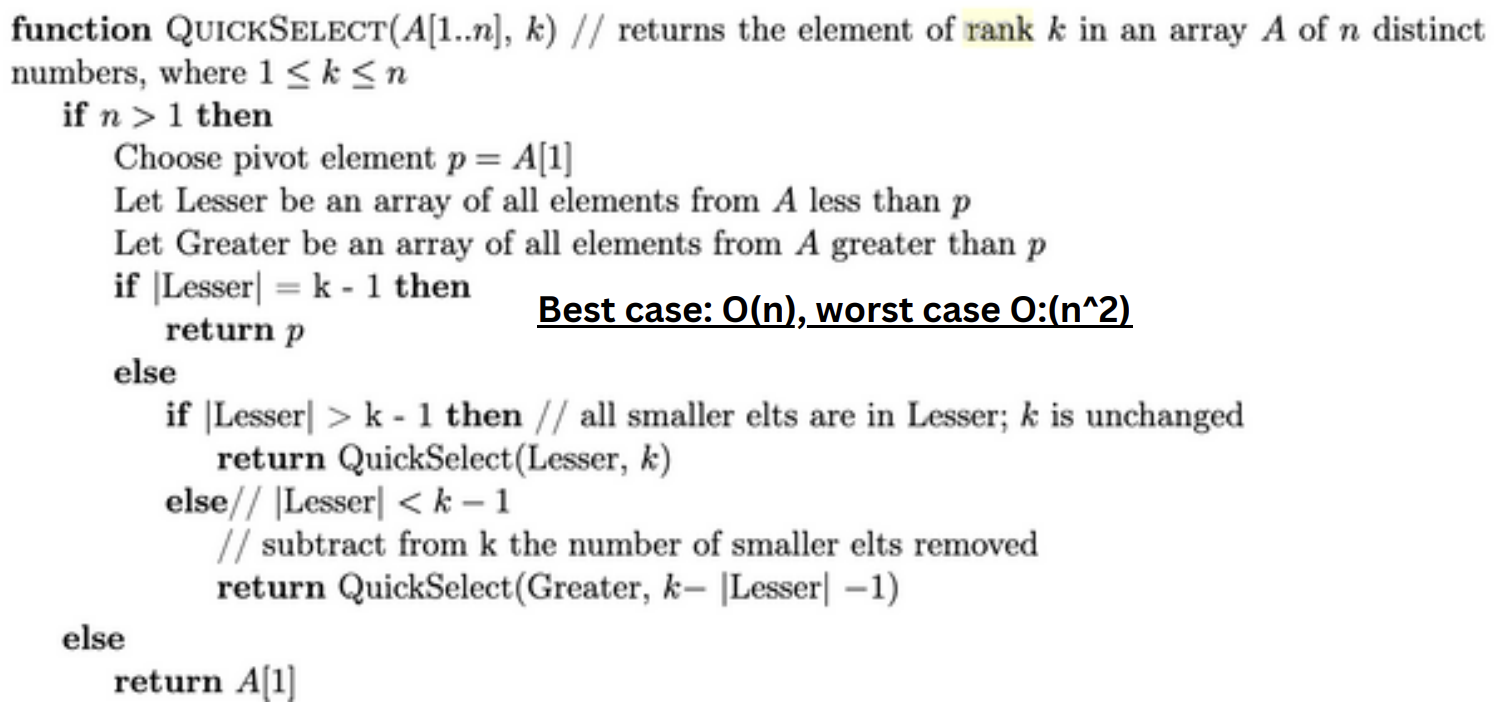
\includegraphics[width=\linewidth]{sheetimages/quickselect.png}

    \hl{Stock market}

    \begin{verbatim}
Algorithm StockMaxProfit(prices)
    S <- 0
    for each point p of P do
        if q.x < p.x or q.y < p.y then
            add p to S
    return S
    \end{verbatim}

    Each company is (x,y) (expected annual dividends, $-10 \leq y \leq 10$ risk, (-) riskier). Dominates when above and to the right. q = (qx,qy) dominates p = (p.x.p.y) if q.x ≥ p.x and qy = p.y. Sort by increasing x then y. Split ½. Right Subproblem: if a point is maximal here, must be maximal in P. Left Subproblem: if a point is maximal here, not automatically maximal in P. If a point in RSP dominates p in LSP, then a point q in RSP with largest y guaranteed to dominate p

    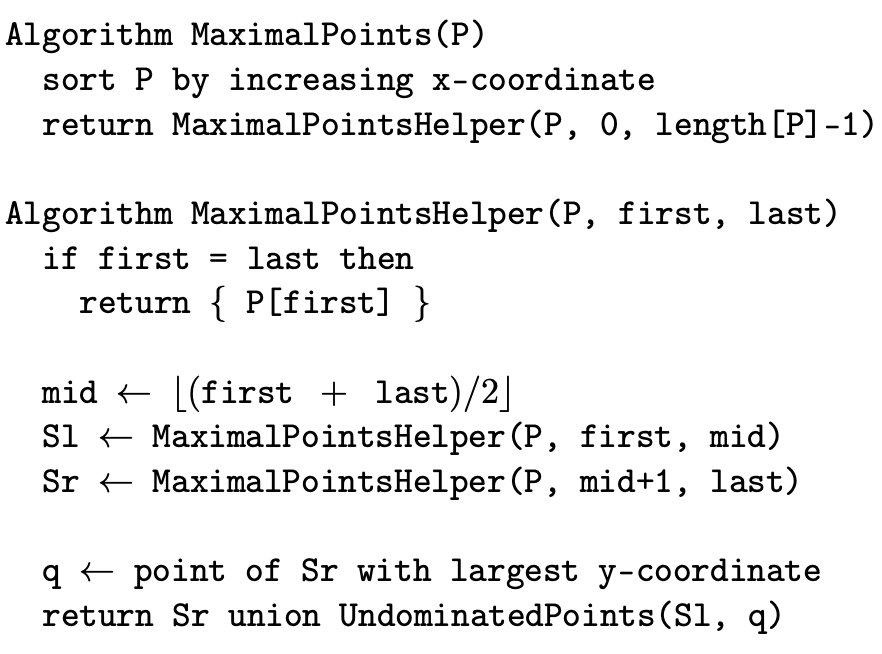
\includegraphics[width=.7\linewidth]{sheetimages/stock2.png}

    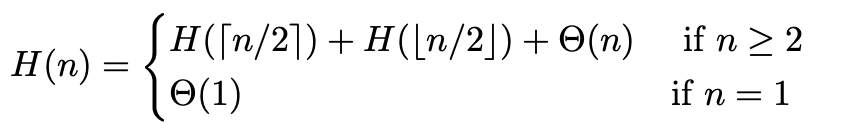
\includegraphics[width=.7\linewidth]{sheetimages/stock3.png} $\in \Theta(n \log n)$

    \hl{Count inversions}

    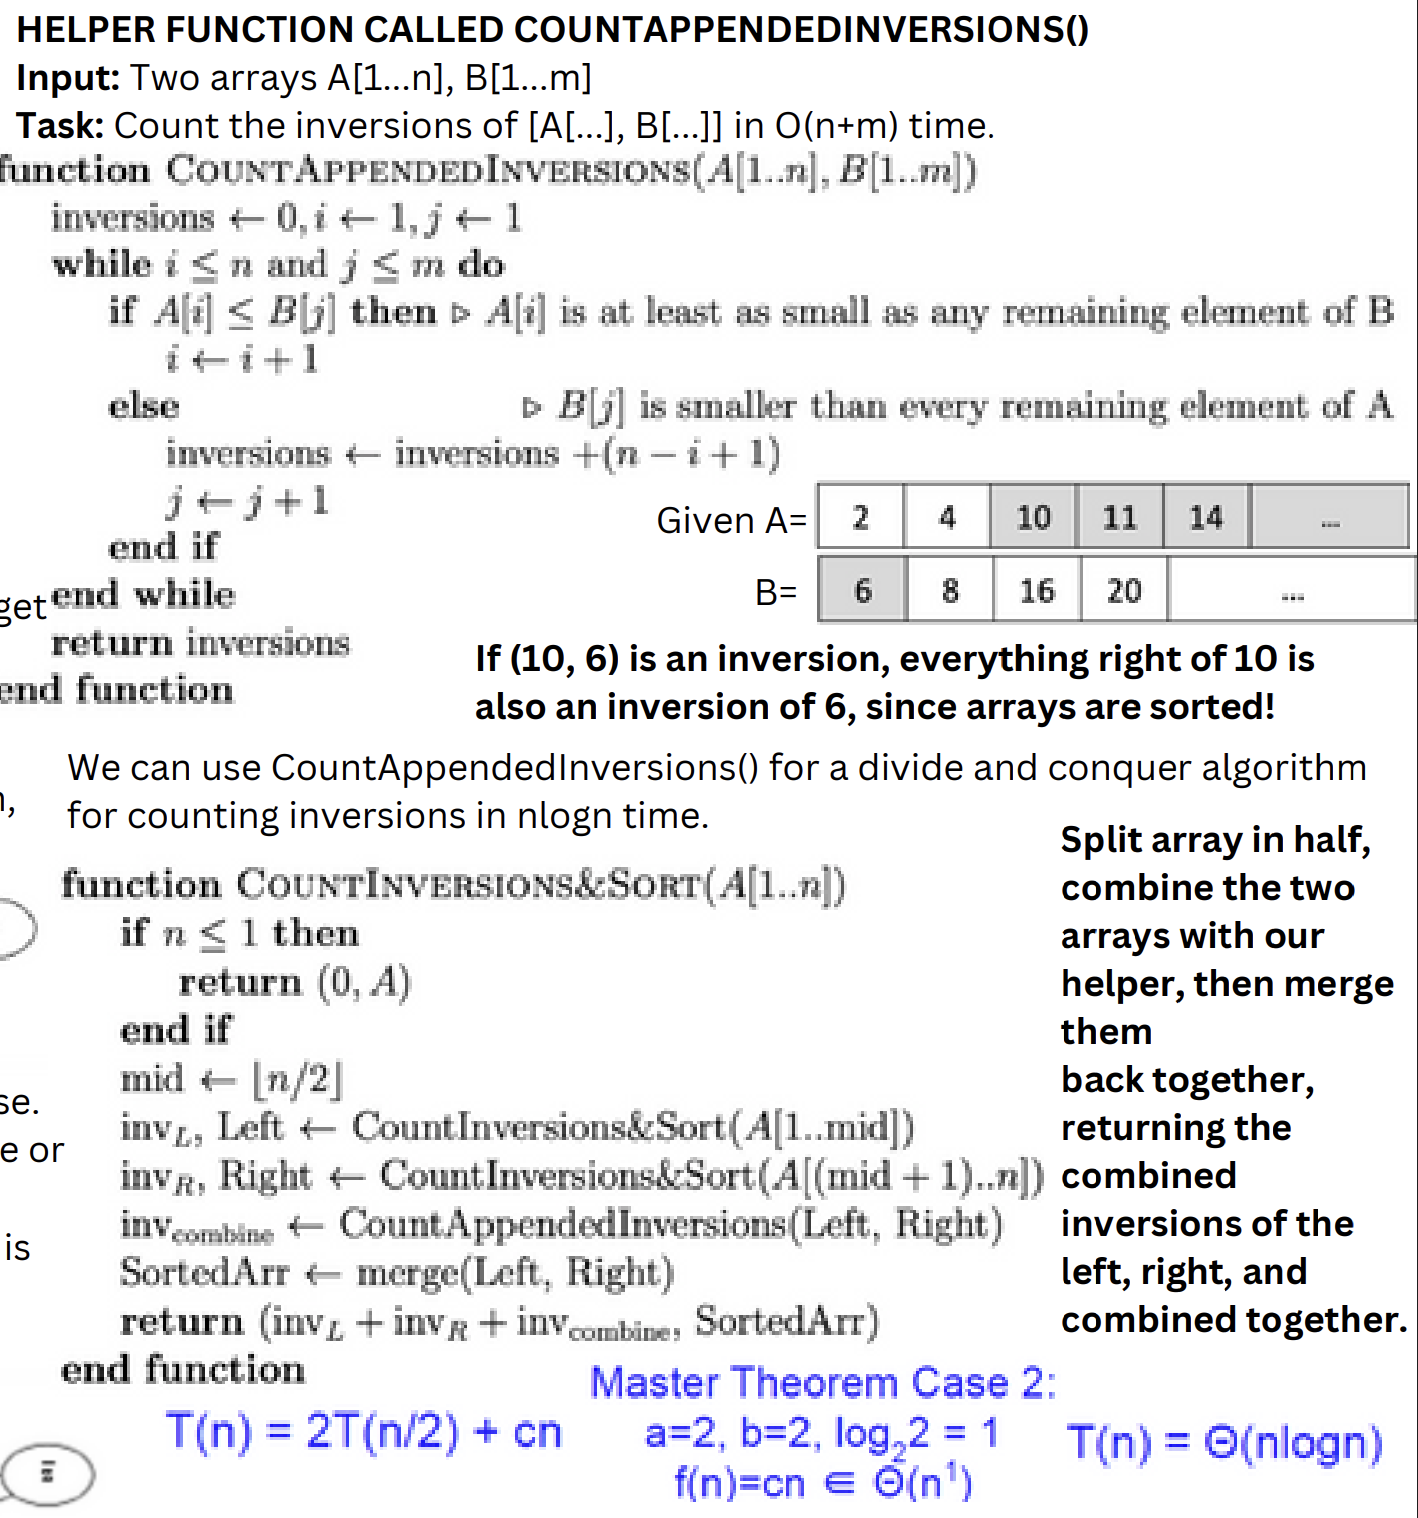
\includegraphics[width=\linewidth]{sheetimages/countinversions.png}

    \section{Resident matching (reduction)}

    The Gale-Shapley algorithm solves the stable matching problem in $O(n^2)$ time. Each employer ranks each applicant in order of preference, and vice versa.

    \begin{verbatim}
Initially all m in M and w in W are free

while (there is a man m who is free && has not proposed to every woman) {
    Choose such a man m
    Let w be the highest-ranked woman in preference list of m 
        to whom m has not proposed to before
    
    if (w is free) { (m,w) are engaged }
    else {
        w is currently engaged to m*
        if (w prefers m* to m) { m remains free }
        else {
            w prefers m to m*
            (m,w) are engaged
            m* is free
        }
    }
}
return the set S of engaged pairs
    \end{verbatim}

    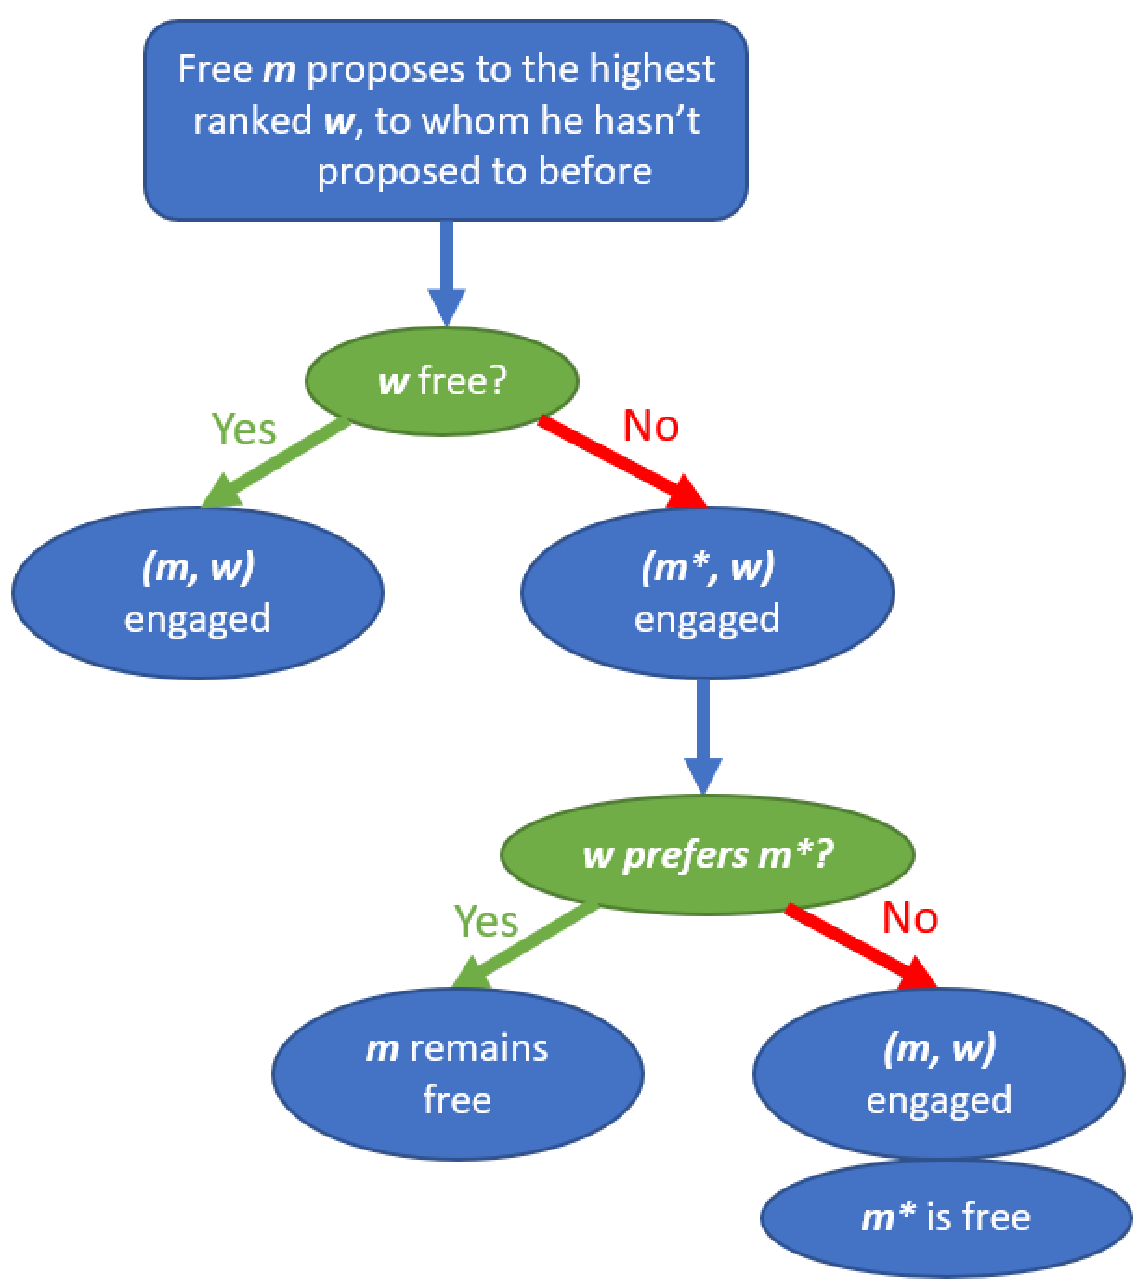
\includegraphics[width=.7\linewidth]{sheetimages/galeshapley.png}

    \textbf{Stable matching}: Input 2 sets of agents of size n, each agent with preference list of other set. Output perfect matching s.t. no blocking pair (m, w) s.t. m prefers w to current and w prefers m to current.

    A \textbf{instability} is:
    \begin{itemize}
        \item \textit{One slot}: a matching where there are two people of different groups who would prefer each other over their current partners.
        \item \textit{Multi-slots}: employer $e$ matched with residents ${a_1, a_2, \ldots, a_k}$, and $a$ matched with $e'$ such that $a$ prefers $e$ over $e'$ and $e$ prefers $a$ over \textbf{$a_k$} (worst member)
    \end{itemize}

    \textbf{RHP:} Input: set of residents R, set of hospitals H, each hospital h has $s(h)$ slots, each agent has preference list over other set. Output: matching s.t. no instabilities.

    Reduction of RHP to SMP:

    \begin{enumerate}
        \item Reduce the Resident Hospital Problem to Stable Matching Prob.
        \item Transform a small instance of RHP into an instance of B.
              \\
              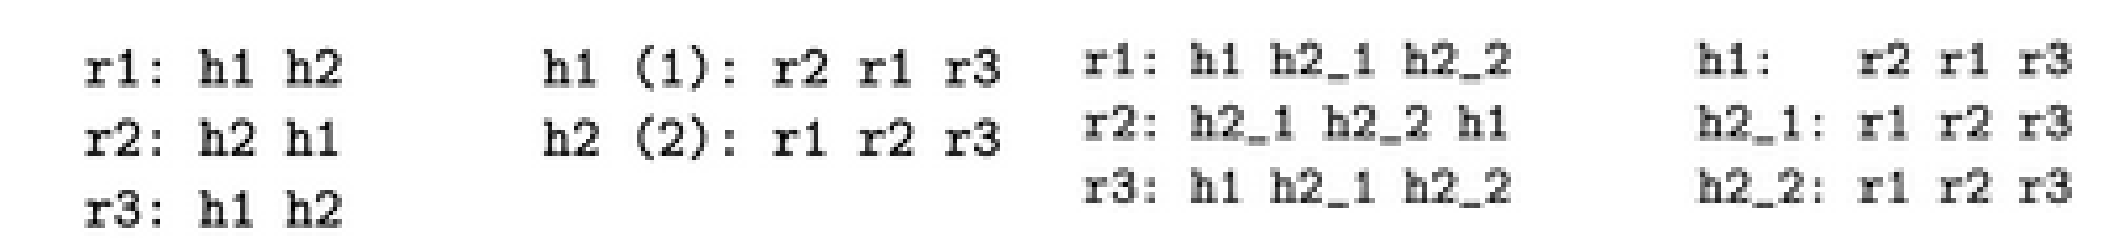
\includegraphics[width=\linewidth]{sheetimages/rhp.png}
        \item Transform a solution from B instance into a solution to the RHP instance.
        \item Design an algorithm to transform any instance I of RHP to an instance of BClone hospitals, with all having same preference list. Once this is done, is SMP instance.
        \item Design an algorithm to transform a solution of B into a solution for RHP.
    \end{enumerate}
    The only thing different about M from a possibly-stable RHP solution wouldbe the subscripts on the hospital-slots. If we erase those, then since each
    hospital-slot had one match and each hospital had s(h) hospital-slots, eachhospital in the RHP solution will now have s(h) matches, as we expect

    \section{Graph}
    \begin{itemize}
        \item \textbf{Path}: ${v1, v2, \cdots , vk}$ such that there exists an edge between consecutive vertices.
        \item \textbf{Hamiltonian Path}: A path that visits each vertex exactly once.
        \item \textbf{Cycle}: A path that starts and ends at the same vertex.
        \item \textbf{Hamiltonian Cycle}: A cycle that visits each vertex exactly once.
        \item \textbf{Connected Graph}: A graph is connected if there is a path between any two vertices.
        \item \textbf{Bipartite Graph}: A graph $G = (V, E)$ is bipartite if the vertex set $V$ can be partitioned into two sets $V_1$ and $V_2$ such that every edge in $E$ has one endpoint in $V_1$ and the other endpoint in $V_2$.
        \item \textbf{Complete Graph}: Number of edges = $\frac{n(n-1)}{2}$
        \item \textbf{Spanning tree}: A spanning tree of a connected, undirected graph is a subgraph that is a tree and connects all the vertices together.
        \item \textbf{Minimum Spanning Tree}: A spanning tree with weight less than or equal to the weight of every other spanning tree. (Solved by Kruskal's and Prim's - P)
    \end{itemize}

    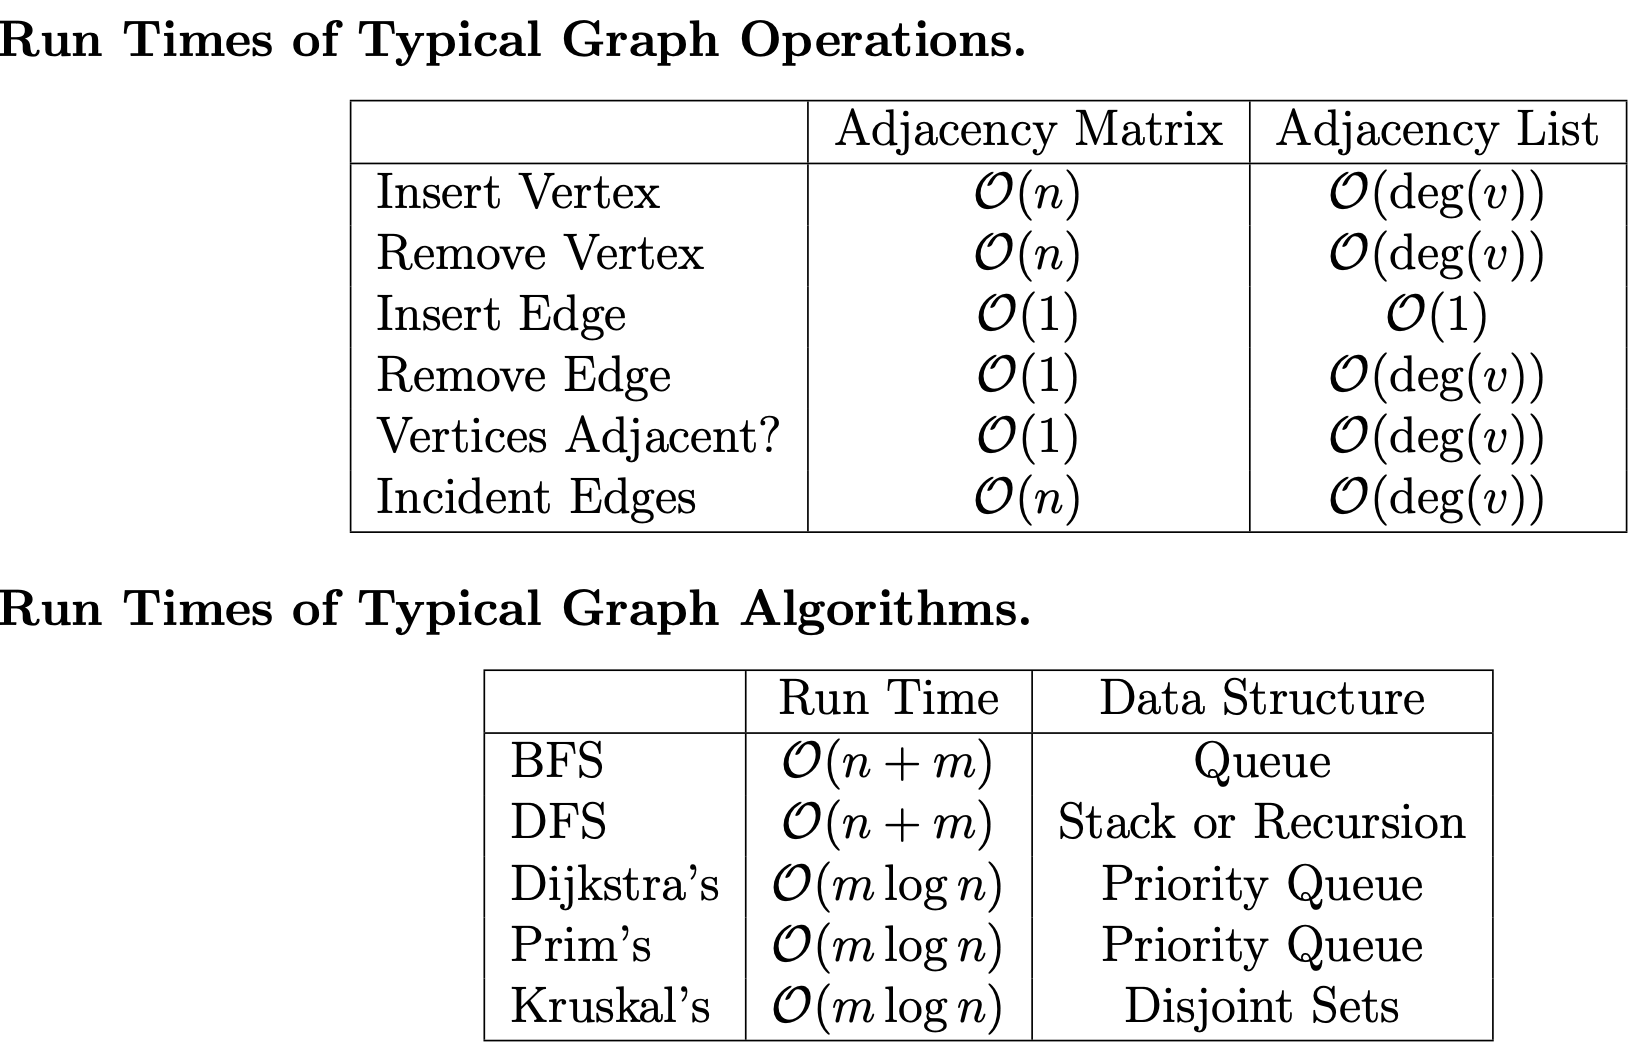
\includegraphics[width=\linewidth]{sheetimages/graphruntime.png}
    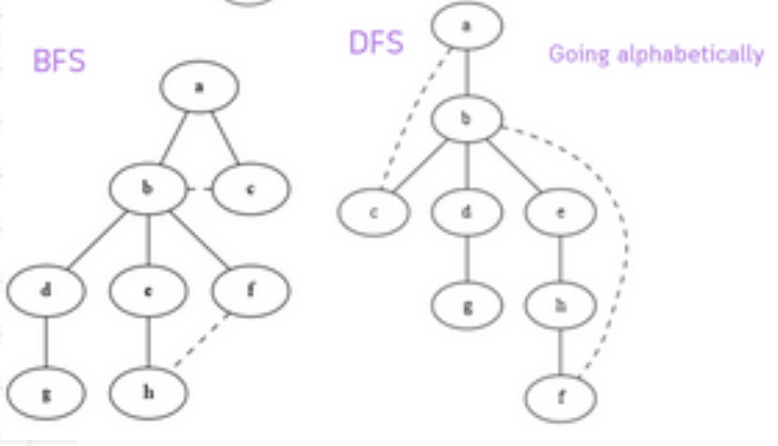
\includegraphics[width=.7\linewidth]{sheetimages/bfsdfs.png}

    \section{Random stuff}

    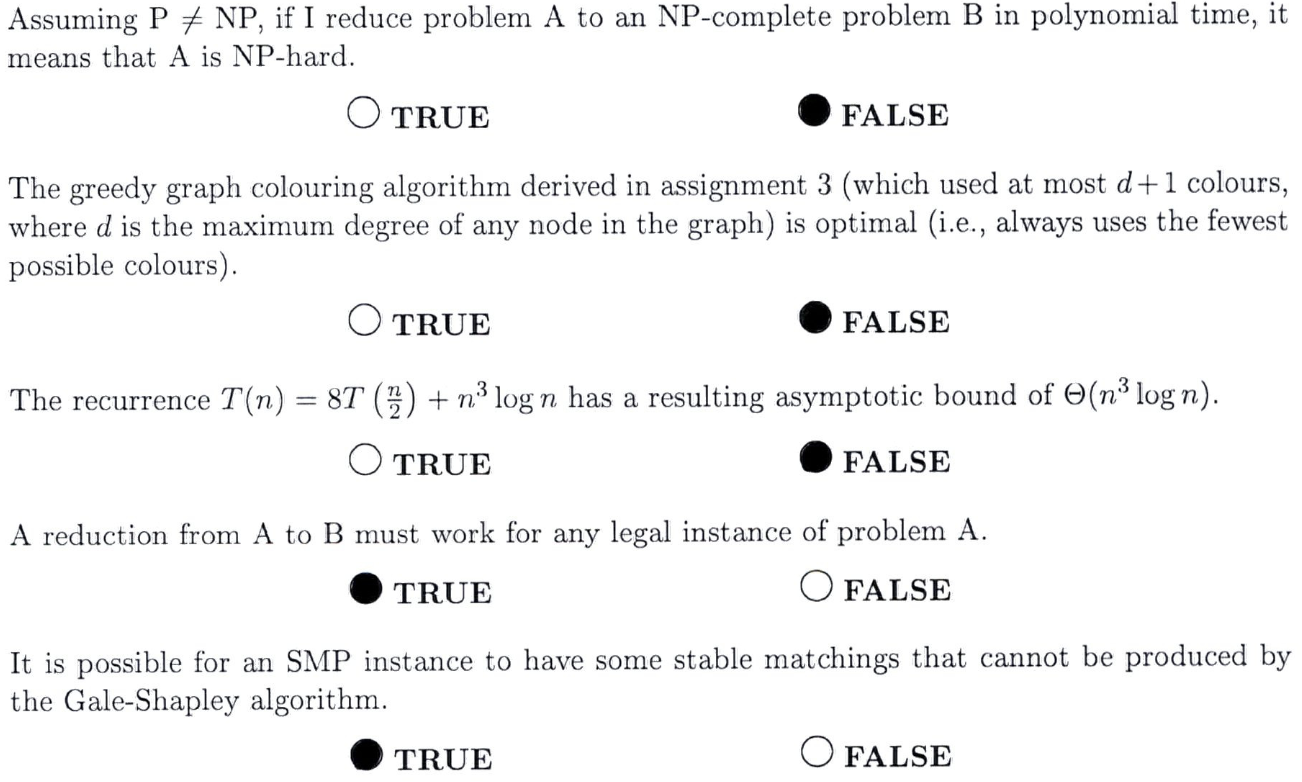
\includegraphics[width=\linewidth]{sheetimages/tf1.png}

    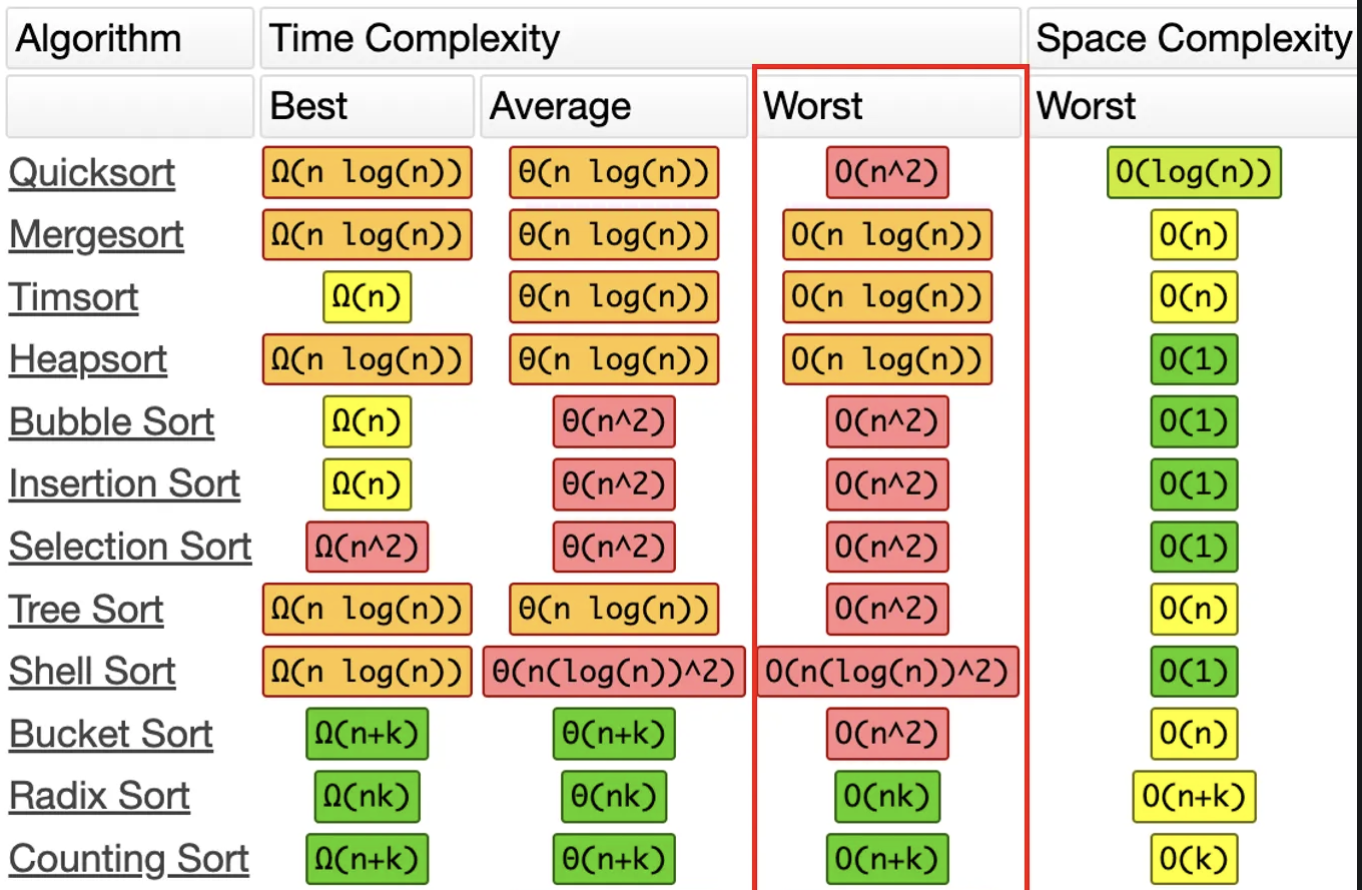
\includegraphics[width=.8\linewidth]{sheetimages/sort.png}

    Quicksort recurrence:

    $T(n)=\begin{cases}\Theta(1)&\text{if }n\leq1\\T(k-1)+T(n-k)+\Theta(n)&\text{if }n>1\end{cases}$

    Mergesort recurrence:

    $T(n)=\begin{cases}\Theta(1)&\text{if }n\leq1\\2T(n/2)+\Theta(n)&\text{if }n>1\end{cases}$

    \vfill
\end{multicols*}
\end{document}